\documentclass[]{fairmeta}
% Option "twocolumn" available, but please prioritize single-column
\usepackage{wrapfig}
\usepackage{hyperref}
\usepackage{url}
\usepackage{algcompatible}
\usepackage{algorithm}
\usepackage{algpseudocode}
\usepackage{graphicx}
\usepackage[T1]{fontenc} 
\usepackage{booktabs}
\usepackage{multirow}
\usepackage{xspace}
\usepackage{float}
\newcommand{\ours}{\textsc{Coconut}\xspace}
\NewDocumentCommand{\shibo}{ mO{} }{\textcolor{cyan}
{\textsuperscript{\textit{Shibo}}\textsf{\textbf{\small[#1]}}}}

\NewDocumentCommand{\andy}{ mO{} }{\textcolor{purple}
{\textsuperscript{\textit{Andy}}\textsf{\textbf{\small[#1]}}}}
\newcommand{\dataset}{ProsQA}
%%%%% NEW MATH DEFINITIONS %%%%%

\usepackage{amsmath,amsfonts,bm}

% Mark sections of captions for referring to divisions of figures
\newcommand{\figleft}{{\em (Left)}}
\newcommand{\figcenter}{{\em (Center)}}
\newcommand{\figright}{{\em (Right)}}
\newcommand{\figtop}{{\em (Top)}}
\newcommand{\figbottom}{{\em (Bottom)}}
\newcommand{\captiona}{{\em (a)}}
\newcommand{\captionb}{{\em (b)}}
\newcommand{\captionc}{{\em (c)}}
\newcommand{\captiond}{{\em (d)}}

% Highlight a newly defined term
\newcommand{\newterm}[1]{{\bf #1}}


% Figure reference, lower-case.
\def\figref#1{figure~\ref{#1}}
% Figure reference, capital. For start of sentence
\def\Figref#1{Figure~\ref{#1}}
\def\twofigref#1#2{figures \ref{#1} and \ref{#2}}
\def\quadfigref#1#2#3#4{figures \ref{#1}, \ref{#2}, \ref{#3} and \ref{#4}}
% Section reference, lower-case.
\def\secref#1{section~\ref{#1}}
% Section reference, capital.
\def\Secref#1{Section~\ref{#1}}
% Reference to two sections.
\def\twosecrefs#1#2{sections \ref{#1} and \ref{#2}}
% Reference to three sections.
\def\secrefs#1#2#3{sections \ref{#1}, \ref{#2} and \ref{#3}}
% Reference to an equation, lower-case.
% \def\eqref#1{equation~\ref{#1}}
\def\eqref#1{(\ref{#1})}
% Reference to an equation, upper case
\def\Eqref#1{Equation~\ref{#1}}
% A raw reference to an equation---avoid using if possible
\def\plaineqref#1{\ref{#1}}
% Reference to a chapter, lower-case.
\def\chapref#1{chapter~\ref{#1}}
% Reference to an equation, upper case.
\def\Chapref#1{Chapter~\ref{#1}}
% Reference to a range of chapters
\def\rangechapref#1#2{chapters\ref{#1}--\ref{#2}}
% Reference to an algorithm, lower-case.
\def\algref#1{algorithm~\ref{#1}}
% Reference to an algorithm, upper case.
\def\Algref#1{Algorithm~\ref{#1}}
\def\twoalgref#1#2{algorithms \ref{#1} and \ref{#2}}
\def\Twoalgref#1#2{Algorithms \ref{#1} and \ref{#2}}
% Reference to a part, lower case
\def\partref#1{part~\ref{#1}}
% Reference to a part, upper case
\def\Partref#1{Part~\ref{#1}}
\def\twopartref#1#2{parts \ref{#1} and \ref{#2}}

\def\ceil#1{\lceil #1 \rceil}
\def\floor#1{\lfloor #1 \rfloor}
\def\1{\bm{1}}
\newcommand{\train}{\mathcal{D}}
\newcommand{\valid}{\mathcal{D_{\mathrm{valid}}}}
\newcommand{\test}{\mathcal{D_{\mathrm{test}}}}

\def\eps{{\epsilon}}


% Random variables
\def\reta{{\textnormal{$\eta$}}}
\def\ra{{\textnormal{a}}}
\def\rb{{\textnormal{b}}}
\def\rc{{\textnormal{c}}}
\def\rd{{\textnormal{d}}}
\def\re{{\textnormal{e}}}
\def\rf{{\textnormal{f}}}
\def\rg{{\textnormal{g}}}
\def\rh{{\textnormal{h}}}
\def\ri{{\textnormal{i}}}
\def\rj{{\textnormal{j}}}
\def\rk{{\textnormal{k}}}
\def\rl{{\textnormal{l}}}
% rm is already a command, just don't name any random variables m
\def\rn{{\textnormal{n}}}
\def\ro{{\textnormal{o}}}
\def\rp{{\textnormal{p}}}
\def\rq{{\textnormal{q}}}
\def\rr{{\textnormal{r}}}
\def\rs{{\textnormal{s}}}
\def\rt{{\textnormal{t}}}
\def\ru{{\textnormal{u}}}
\def\rv{{\textnormal{v}}}
\def\rw{{\textnormal{w}}}
\def\rx{{\textnormal{x}}}
\def\ry{{\textnormal{y}}}
\def\rz{{\textnormal{z}}}

% Random vectors
\def\rvepsilon{{\mathbf{\epsilon}}}
\def\rvtheta{{\mathbf{\theta}}}
\def\rva{{\mathbf{a}}}
\def\rvb{{\mathbf{b}}}
\def\rvc{{\mathbf{c}}}
\def\rvd{{\mathbf{d}}}
\def\rve{{\mathbf{e}}}
\def\rvf{{\mathbf{f}}}
\def\rvg{{\mathbf{g}}}
\def\rvh{{\mathbf{h}}}
\def\rvu{{\mathbf{i}}}
\def\rvj{{\mathbf{j}}}
\def\rvk{{\mathbf{k}}}
\def\rvl{{\mathbf{l}}}
\def\rvm{{\mathbf{m}}}
\def\rvn{{\mathbf{n}}}
\def\rvo{{\mathbf{o}}}
\def\rvp{{\mathbf{p}}}
\def\rvq{{\mathbf{q}}}
\def\rvr{{\mathbf{r}}}
\def\rvs{{\mathbf{s}}}
\def\rvt{{\mathbf{t}}}
\def\rvu{{\mathbf{u}}}
\def\rvv{{\mathbf{v}}}
\def\rvw{{\mathbf{w}}}
\def\rvx{{\mathbf{x}}}
\def\rvy{{\mathbf{y}}}
\def\rvz{{\mathbf{z}}}

% Elements of random vectors
\def\erva{{\textnormal{a}}}
\def\ervb{{\textnormal{b}}}
\def\ervc{{\textnormal{c}}}
\def\ervd{{\textnormal{d}}}
\def\erve{{\textnormal{e}}}
\def\ervf{{\textnormal{f}}}
\def\ervg{{\textnormal{g}}}
\def\ervh{{\textnormal{h}}}
\def\ervi{{\textnormal{i}}}
\def\ervj{{\textnormal{j}}}
\def\ervk{{\textnormal{k}}}
\def\ervl{{\textnormal{l}}}
\def\ervm{{\textnormal{m}}}
\def\ervn{{\textnormal{n}}}
\def\ervo{{\textnormal{o}}}
\def\ervp{{\textnormal{p}}}
\def\ervq{{\textnormal{q}}}
\def\ervr{{\textnormal{r}}}
\def\ervs{{\textnormal{s}}}
\def\ervt{{\textnormal{t}}}
\def\ervu{{\textnormal{u}}}
\def\ervv{{\textnormal{v}}}
\def\ervw{{\textnormal{w}}}
\def\ervx{{\textnormal{x}}}
\def\ervy{{\textnormal{y}}}
\def\ervz{{\textnormal{z}}}

% Random matrices
\def\rmA{{\mathbf{A}}}
\def\rmB{{\mathbf{B}}}
\def\rmC{{\mathbf{C}}}
\def\rmD{{\mathbf{D}}}
\def\rmE{{\mathbf{E}}}
\def\rmF{{\mathbf{F}}}
\def\rmG{{\mathbf{G}}}
\def\rmH{{\mathbf{H}}}
\def\rmI{{\mathbf{I}}}
\def\rmJ{{\mathbf{J}}}
\def\rmK{{\mathbf{K}}}
\def\rmL{{\mathbf{L}}}
\def\rmM{{\mathbf{M}}}
\def\rmN{{\mathbf{N}}}
\def\rmO{{\mathbf{O}}}
\def\rmP{{\mathbf{P}}}
\def\rmQ{{\mathbf{Q}}}
\def\rmR{{\mathbf{R}}}
\def\rmS{{\mathbf{S}}}
\def\rmT{{\mathbf{T}}}
\def\rmU{{\mathbf{U}}}
\def\rmV{{\mathbf{V}}}
\def\rmW{{\mathbf{W}}}
\def\rmX{{\mathbf{X}}}
\def\rmY{{\mathbf{Y}}}
\def\rmZ{{\mathbf{Z}}}

% Elements of random matrices
\def\ermA{{\textnormal{A}}}
\def\ermB{{\textnormal{B}}}
\def\ermC{{\textnormal{C}}}
\def\ermD{{\textnormal{D}}}
\def\ermE{{\textnormal{E}}}
\def\ermF{{\textnormal{F}}}
\def\ermG{{\textnormal{G}}}
\def\ermH{{\textnormal{H}}}
\def\ermI{{\textnormal{I}}}
\def\ermJ{{\textnormal{J}}}
\def\ermK{{\textnormal{K}}}
\def\ermL{{\textnormal{L}}}
\def\ermM{{\textnormal{M}}}
\def\ermN{{\textnormal{N}}}
\def\ermO{{\textnormal{O}}}
\def\ermP{{\textnormal{P}}}
\def\ermQ{{\textnormal{Q}}}
\def\ermR{{\textnormal{R}}}
\def\ermS{{\textnormal{S}}}
\def\ermT{{\textnormal{T}}}
\def\ermU{{\textnormal{U}}}
\def\ermV{{\textnormal{V}}}
\def\ermW{{\textnormal{W}}}
\def\ermX{{\textnormal{X}}}
\def\ermY{{\textnormal{Y}}}
\def\ermZ{{\textnormal{Z}}}

% Vectors
\def\vzero{{\bm{0}}}
\def\vone{{\bm{1}}}
\def\vmu{{\bm{\mu}}}
\def\vtheta{{\bm{\theta}}}
\def\va{{\bm{a}}}
\def\vb{{\bm{b}}}
\def\vc{{\bm{c}}}
\def\vd{{\bm{d}}}
\def\ve{{\bm{e}}}
\def\vf{{\bm{f}}}
\def\vg{{\bm{g}}}
\def\vh{{\bm{h}}}
\def\vi{{\bm{i}}}
\def\vj{{\bm{j}}}
\def\vk{{\bm{k}}}
\def\vl{{\bm{l}}}
\def\vm{{\bm{m}}}
\def\vn{{\bm{n}}}
\def\vo{{\bm{o}}}
\def\vp{{\bm{p}}}
\def\vq{{\bm{q}}}
\def\vr{{\bm{r}}}
\def\vs{{\bm{s}}}
\def\vt{{\bm{t}}}
\def\vu{{\bm{u}}}
\def\vv{{\bm{v}}}
\def\vw{{\bm{w}}}
\def\vx{{\bm{x}}}
\def\vy{{\bm{y}}}
\def\vz{{\bm{z}}}

% Elements of vectors
\def\evalpha{{\alpha}}
\def\evbeta{{\beta}}
\def\evepsilon{{\epsilon}}
\def\evlambda{{\lambda}}
\def\evomega{{\omega}}
\def\evmu{{\mu}}
\def\evpsi{{\psi}}
\def\evsigma{{\sigma}}
\def\evtheta{{\theta}}
\def\eva{{a}}
\def\evb{{b}}
\def\evc{{c}}
\def\evd{{d}}
\def\eve{{e}}
\def\evf{{f}}
\def\evg{{g}}
\def\evh{{h}}
\def\evi{{i}}
\def\evj{{j}}
\def\evk{{k}}
\def\evl{{l}}
\def\evm{{m}}
\def\evn{{n}}
\def\evo{{o}}
\def\evp{{p}}
\def\evq{{q}}
\def\evr{{r}}
\def\evs{{s}}
\def\evt{{t}}
\def\evu{{u}}
\def\evv{{v}}
\def\evw{{w}}
\def\evx{{x}}
\def\evy{{y}}
\def\evz{{z}}

% Matrix
\def\mA{{\bm{A}}}
\def\mB{{\bm{B}}}
\def\mC{{\bm{C}}}
\def\mD{{\bm{D}}}
\def\mE{{\bm{E}}}
\def\mF{{\bm{F}}}
\def\mG{{\bm{G}}}
\def\mH{{\bm{H}}}
\def\mI{{\bm{I}}}
\def\mJ{{\bm{J}}}
\def\mK{{\bm{K}}}
\def\mL{{\bm{L}}}
\def\mM{{\bm{M}}}
\def\mN{{\bm{N}}}
\def\mO{{\bm{O}}}
\def\mP{{\bm{P}}}
\def\mQ{{\bm{Q}}}
\def\mR{{\bm{R}}}
\def\mS{{\bm{S}}}
\def\mT{{\bm{T}}}
\def\mU{{\bm{U}}}
\def\mV{{\bm{V}}}
\def\mW{{\bm{W}}}
\def\mX{{\bm{X}}}
\def\mY{{\bm{Y}}}
\def\mZ{{\bm{Z}}}
\def\mBeta{{\bm{\beta}}}
\def\mPhi{{\bm{\Phi}}}
\def\mLambda{{\bm{\Lambda}}}
\def\mSigma{{\bm{\Sigma}}}

% Tensor
\DeclareMathAlphabet{\mathsfit}{\encodingdefault}{\sfdefault}{m}{sl}
\SetMathAlphabet{\mathsfit}{bold}{\encodingdefault}{\sfdefault}{bx}{n}
\newcommand{\tens}[1]{\bm{\mathsfit{#1}}}
\def\tA{{\tens{A}}}
\def\tB{{\tens{B}}}
\def\tC{{\tens{C}}}
\def\tD{{\tens{D}}}
\def\tE{{\tens{E}}}
\def\tF{{\tens{F}}}
\def\tG{{\tens{G}}}
\def\tH{{\tens{H}}}
\def\tI{{\tens{I}}}
\def\tJ{{\tens{J}}}
\def\tK{{\tens{K}}}
\def\tL{{\tens{L}}}
\def\tM{{\tens{M}}}
\def\tN{{\tens{N}}}
\def\tO{{\tens{O}}}
\def\tP{{\tens{P}}}
\def\tQ{{\tens{Q}}}
\def\tR{{\tens{R}}}
\def\tS{{\tens{S}}}
\def\tT{{\tens{T}}}
\def\tU{{\tens{U}}}
\def\tV{{\tens{V}}}
\def\tW{{\tens{W}}}
\def\tX{{\tens{X}}}
\def\tY{{\tens{Y}}}
\def\tZ{{\tens{Z}}}


% Graph
\def\gA{{\mathcal{A}}}
\def\gB{{\mathcal{B}}}
\def\gC{{\mathcal{C}}}
\def\gD{{\mathcal{D}}}
\def\gE{{\mathcal{E}}}
\def\gF{{\mathcal{F}}}
\def\gG{{\mathcal{G}}}
\def\gH{{\mathcal{H}}}
\def\gI{{\mathcal{I}}}
\def\gJ{{\mathcal{J}}}
\def\gK{{\mathcal{K}}}
\def\gL{{\mathcal{L}}}
\def\gM{{\mathcal{M}}}
\def\gN{{\mathcal{N}}}
\def\gO{{\mathcal{O}}}
\def\gP{{\mathcal{P}}}
\def\gQ{{\mathcal{Q}}}
\def\gR{{\mathcal{R}}}
\def\gS{{\mathcal{S}}}
\def\gT{{\mathcal{T}}}
\def\gU{{\mathcal{U}}}
\def\gV{{\mathcal{V}}}
\def\gW{{\mathcal{W}}}
\def\gX{{\mathcal{X}}}
\def\gY{{\mathcal{Y}}}
\def\gZ{{\mathcal{Z}}}

% Sets
\def\sA{{\mathbb{A}}}
\def\sB{{\mathbb{B}}}
\def\sC{{\mathbb{C}}}
\def\sD{{\mathbb{D}}}
% Don't use a set called E, because this would be the same as our symbol
% for expectation.
\def\sF{{\mathbb{F}}}
\def\sG{{\mathbb{G}}}
\def\sH{{\mathbb{H}}}
\def\sI{{\mathbb{I}}}
\def\sJ{{\mathbb{J}}}
\def\sK{{\mathbb{K}}}
\def\sL{{\mathbb{L}}}
\def\sM{{\mathbb{M}}}
\def\sN{{\mathbb{N}}}
\def\sO{{\mathbb{O}}}
\def\sP{{\mathbb{P}}}
\def\sQ{{\mathbb{Q}}}
\def\sR{{\mathbb{R}}}
\def\sS{{\mathbb{S}}}
\def\sT{{\mathbb{T}}}
\def\sU{{\mathbb{U}}}
\def\sV{{\mathbb{V}}}
\def\sW{{\mathbb{W}}}
\def\sX{{\mathbb{X}}}
\def\sY{{\mathbb{Y}}}
\def\sZ{{\mathbb{Z}}}

% Entries of a matrix
\def\emLambda{{\Lambda}}
\def\emA{{A}}
\def\emB{{B}}
\def\emC{{C}}
\def\emD{{D}}
\def\emE{{E}}
\def\emF{{F}}
\def\emG{{G}}
\def\emH{{H}}
\def\emI{{I}}
\def\emJ{{J}}
\def\emK{{K}}
\def\emL{{L}}
\def\emM{{M}}
\def\emN{{N}}
\def\emO{{O}}
\def\emP{{P}}
\def\emQ{{Q}}
\def\emR{{R}}
\def\emS{{S}}
\def\emT{{T}}
\def\emU{{U}}
\def\emV{{V}}
\def\emW{{W}}
\def\emX{{X}}
\def\emY{{Y}}
\def\emZ{{Z}}
\def\emSigma{{\Sigma}}

% entries of a tensor
% Same font as tensor, without \bm wrapper
\newcommand{\etens}[1]{\mathsfit{#1}}
\def\etLambda{{\etens{\Lambda}}}
\def\etA{{\etens{A}}}
\def\etB{{\etens{B}}}
\def\etC{{\etens{C}}}
\def\etD{{\etens{D}}}
\def\etE{{\etens{E}}}
\def\etF{{\etens{F}}}
\def\etG{{\etens{G}}}
\def\etH{{\etens{H}}}
\def\etI{{\etens{I}}}
\def\etJ{{\etens{J}}}
\def\etK{{\etens{K}}}
\def\etL{{\etens{L}}}
\def\etM{{\etens{M}}}
\def\etN{{\etens{N}}}
\def\etO{{\etens{O}}}
\def\etP{{\etens{P}}}
\def\etQ{{\etens{Q}}}
\def\etR{{\etens{R}}}
\def\etS{{\etens{S}}}
\def\etT{{\etens{T}}}
\def\etU{{\etens{U}}}
\def\etV{{\etens{V}}}
\def\etW{{\etens{W}}}
\def\etX{{\etens{X}}}
\def\etY{{\etens{Y}}}
\def\etZ{{\etens{Z}}}

% The true underlying data generating distribution
\newcommand{\pdata}{p_{\rm{data}}}
% The empirical distribution defined by the training set
\newcommand{\ptrain}{\hat{p}_{\rm{data}}}
\newcommand{\Ptrain}{\hat{P}_{\rm{data}}}
% The model distribution
\newcommand{\pmodel}{p_{\rm{model}}}
\newcommand{\Pmodel}{P_{\rm{model}}}
\newcommand{\ptildemodel}{\tilde{p}_{\rm{model}}}
% Stochastic autoencoder distributions
\newcommand{\pencode}{p_{\rm{encoder}}}
\newcommand{\pdecode}{p_{\rm{decoder}}}
\newcommand{\precons}{p_{\rm{reconstruct}}}

\newcommand{\laplace}{\mathrm{Laplace}} % Laplace distribution

\newcommand{\E}{\mathbb{E}}
\newcommand{\Ls}{\mathcal{L}}
\newcommand{\R}{\mathbb{R}}
\newcommand{\emp}{\tilde{p}}
\newcommand{\lr}{\alpha}
\newcommand{\reg}{\lambda}
\newcommand{\rect}{\mathrm{rectifier}}
\newcommand{\softmax}{\mathrm{softmax}}
\newcommand{\sigmoid}{\sigma}
\newcommand{\softplus}{\zeta}
\newcommand{\KL}{D_{\mathrm{KL}}}
\newcommand{\Var}{\mathrm{Var}}
\newcommand{\standarderror}{\mathrm{SE}}
\newcommand{\Cov}{\mathrm{Cov}}
% Wolfram Mathworld says $L^2$ is for function spaces and $\ell^2$ is for vectors
% But then they seem to use $L^2$ for vectors throughout the site, and so does
% wikipedia.
\newcommand{\normlzero}{L^0}
\newcommand{\normlone}{L^1}
\newcommand{\normltwo}{L^2}
\newcommand{\normlp}{L^p}
\newcommand{\normmax}{L^\infty}

\newcommand{\parents}{Pa} % See usage in notation.tex. Chosen to match Daphne's book.

\DeclareMathOperator*{\argmax}{arg\,max}
\DeclareMathOperator*{\argmin}{arg\,min}

\DeclareMathOperator{\sign}{sign}
\DeclareMathOperator{\Tr}{Tr}
\let\ab\allowbreak

 
\title{Training Large Language Models to Reason in a Continuous Latent Space}

\author[1,2,*]{Shibo Hao}
\author[1]{Sainbayar Sukhbaatar}
\author[1]{DiJia Su}
\author[1]{Xian Li}
\author[2]{Zhiting Hu}
\author[1]{Jason Weston}
\author[1]{Yuandong Tian}

\affiliation[1]{FAIR at Meta}
\affiliation[2]{UC San Diego}

\contribution[*]{Work done at Meta}
%\contribution[\dagger]{Joint last author}

\abstract{
Large language models (LLMs) are restricted to reason in the ``language space'', where they typically express the reasoning process with a chain-of-thought (CoT) to solve a complex reasoning problem. However, we argue that language space may not always be optimal for reasoning. For example, most word tokens are primarily for textual coherence and not essential for reasoning, while some critical tokens require complex planning and pose huge challenges to LLMs. To explore the potential of LLM reasoning in an unrestricted latent space instead of using natural language, we introduce a new paradigm \ours (\underline{C}hain \underline{o}f \underline{Con}tin\underline{u}ous \underline{T}hought). We utilize the last hidden state of the LLM as a representation of the reasoning state (termed ``continuous thought''). Rather than decoding this into a word token, we feed it back to the LLM as the subsequent input embedding directly in the continuous space. Experiments show that \ours can effectively augment the LLM on several reasoning tasks. This novel latent reasoning paradigm leads to emergent advanced reasoning patterns: the continuous thought can encode multiple alternative next reasoning steps, allowing the model to perform a breadth-first search (BFS) to solve the problem, rather than prematurely committing to a single deterministic path like CoT. \ours{} outperforms CoT in certain logical reasoning tasks that require substantial backtracking during planning, with fewer thinking tokens during inference. 
These findings demonstrate the promise of latent reasoning and offer valuable insights for future research.  
%It even outperforms CoT in certain logical reasoning tasks that require substantial planning, despite generating fewer tokens during inference. Interestingly, we observe an advanced reasoning pattern emerging from latent reasoning: the continuous thought can encode multiple potential next reasoning steps, allowing the model to perform a breadth-first search (BFS) to solve the problem, rather than prematurely committing to a single deterministic path like CoT. These findings demonstrate the promise of latent reasoning and offer valuable insights for future research on latent reasoning methods.
}

\date{\today}
%\correspondence{First Author at \email{first.author@meta.com}}

% You can add additional metadata fields as follows 
%\metadata[Code]{\url{https://github.com/facebookresearch/repo}}
%\metadata[Blogpost]{\url{https://ai.meta.com/blog/?page=1}}

\begin{document}

\maketitle

\section{Introduction}
\label{section:intro}
Large language models (LLMs) have demonstrated remarkable reasoning abilities, emerging from extensive pretraining on human languages~\citep{dubey2024llama, achiam2023gpt}. While next token prediction is an effective training objective, it imposes a fundamental constraint on the LLM as a reasoning machine: the explicit reasoning process of LLMs must be generated in word tokens. For example, a prevalent approach, known as chain-of-thought (CoT) reasoning~\citep{wei2022chain}, involves prompting or training LLMs to generate solutions step-by-step using natural language. However, this is in stark contrast to certain human cognition results. Neuroimaging studies have consistently shown that the language network -- a set of brain regions responsible for language comprehension and production -- remains largely inactive during various reasoning tasks ~\citep{amalric2019distinct, monti2012thought, monti2007functional, monti2009boundaries, fedorenko2011functional}. Further evidence indicates that human language is optimized for communication rather than reasoning~\citep{fedorenko2024language}.

A significant issue arises when LLMs use language for reasoning: the amount of reasoning required for each particular reasoning token varies greatly, yet current LLM architectures allocate nearly the same computing budget for predicting every token. Most tokens in a reasoning chain are generated solely for fluency, contributing little to the actual reasoning process. On the contrary, some critical tokens require complex planning and pose huge challenges to LLMs. While previous work has attempted to fix these problems by prompting LLMs to generate succinct reasoning chains~\citep{madaan2022text}, or performing additional reasoning before generating some critical tokens~\citep{zelikman2024quiet}, these solutions remain constrained within the language space and do not solve the fundamental problems. On the contrary, it would be ideal for LLMs to have the freedom to reason without any language constraints, and then translate their findings into language only when necessary.


% \end{wrapfigure}

\begin{figure}
    \centering
    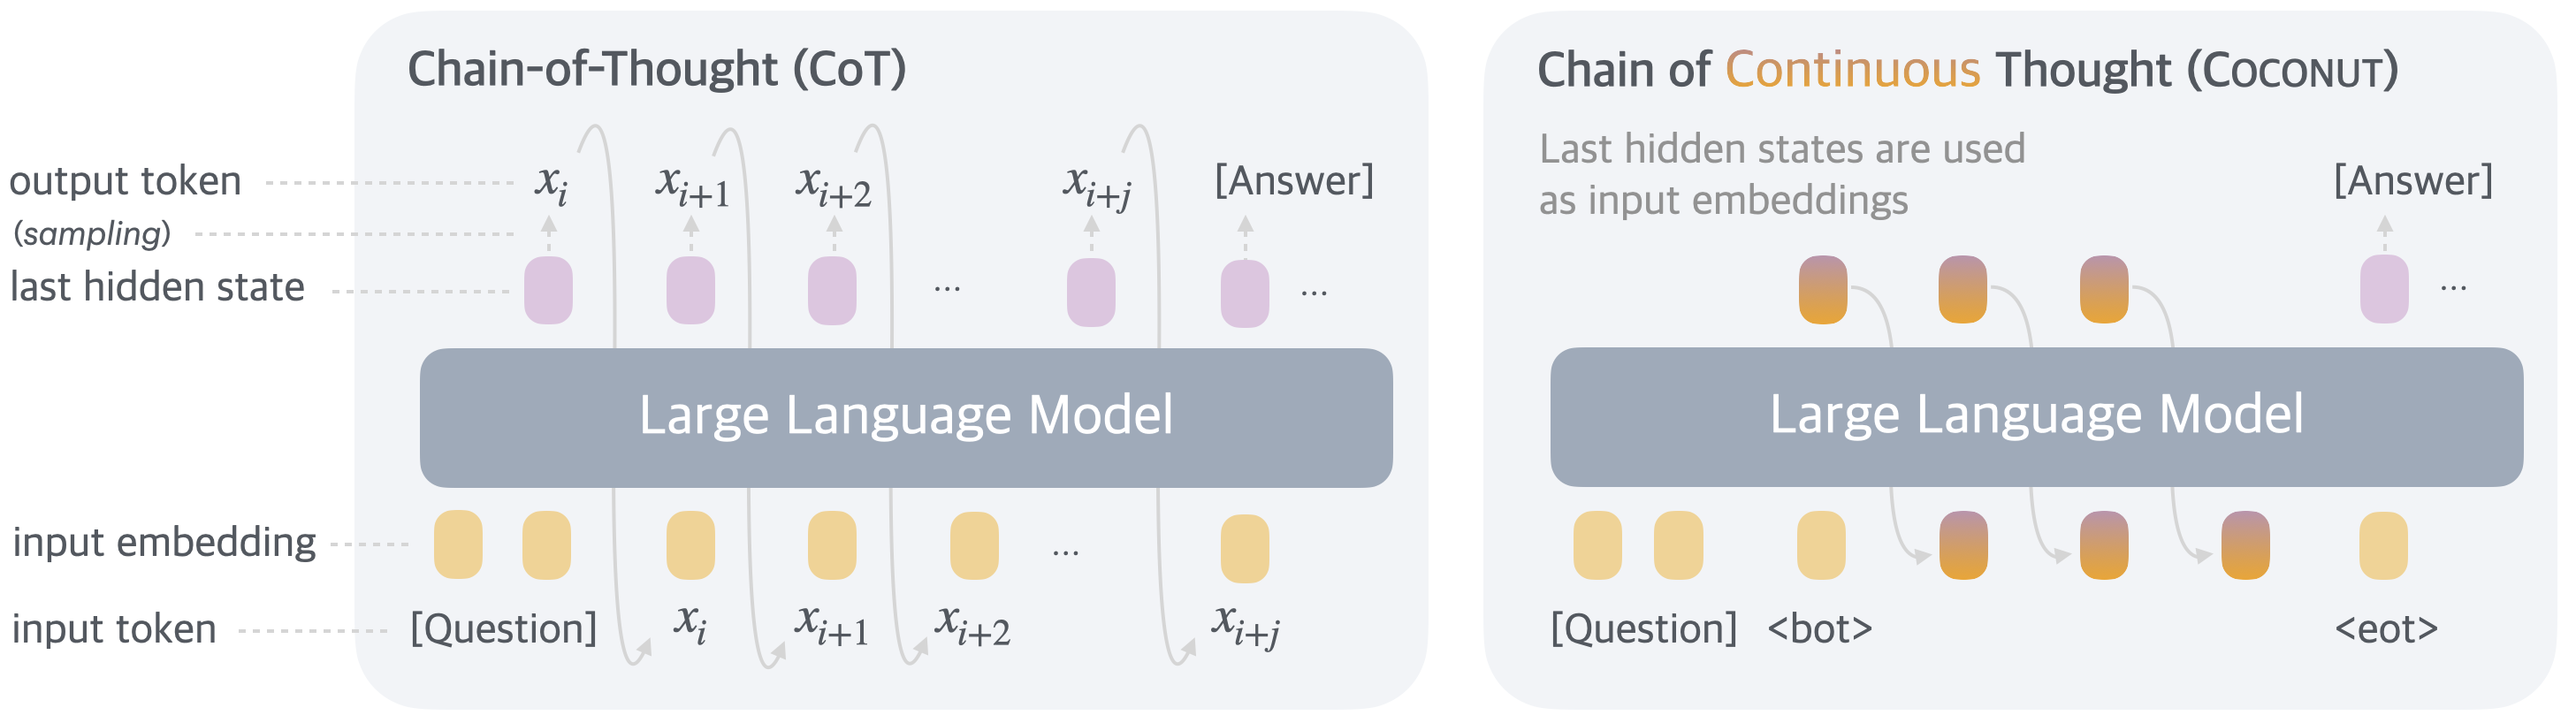
\includegraphics[width=\linewidth]{figures/figure_1_meta_3.png}
    %\vspace{-5pt}
    \caption{A comparison of Chain of Continuous Thought (\ours) with Chain-of-Thought (CoT). In CoT, the model generates the reasoning process as a word token sequence (e.g., $[x_{i}, x_{i+1}, ..., x_{i+j}]$ in the figure). \ours  regards the last hidden state as a representation of the reasoning state (termed ``continuous thought''), and directly uses it as the next input embedding. This allows the LLM to reason in an unrestricted latent space instead of a language space.}
    \label{fig:motivation}
    %\vspace{-5pt}
\end{figure}

In this work we instead explore LLM reasoning in a latent space by introducing a novel paradigm, \ours (Chain of Continuous Thought). It involves a simple modification to the traditional CoT process: instead of mapping between hidden states and language tokens using the language model head and embedding layer, \ours directly feeds the last hidden state (a continuous thought) as the input embedding for the next token (Figure~\ref{fig:motivation}). This modification frees the reasoning from being within the language space, and the system can be optimized end-to-end by gradient descent, as continuous thoughts are fully differentiable. To enhance the training of latent reasoning, we employ a multi-stage training strategy inspired by \citet{deng2024explicit}, which effectively utilizes language reasoning chains to guide the training process.

Interestingly, our proposed paradigm leads to an efficient reasoning pattern. % By manipulating the \ours model to switch between latent reasoning and language reasoning, we are able to unveil the latent reasoning process. 
Unlike language-based reasoning, continuous thoughts in \ours can encode multiple potential next steps simultaneously, allowing for a reasoning process akin to breadth-first search (BFS). While the model may not initially make the correct decision, it can maintain many possible options within the continuous thoughts and progressively eliminate incorrect paths through reasoning, guided by some implicit value functions. This advanced reasoning mechanism surpasses traditional CoT, even though the model is not explicitly trained or instructed to operate in this manner, as seen in previous works \citep{yao2023tree, hao2023reasoning}.

%\shibo{needs to be polished } 
Experimentally, \ours successfully enhances the reasoning capabilities of LLMs. For math reasoning (GSM8k,~\citealp{cobbe2021training}), using continuous thoughts is shown to be beneficial to reasoning accuracy, mirroring the effects of language reasoning chains. This indicates the potential to scale and solve increasingly challenging problems by chaining more continuous thoughts. On logical reasoning including ProntoQA~\citep{saparov2022language}, and our newly proposed ProsQA (Section~\ref{sec:prosqa}) which requires stronger planning ability, \ours and some of its variants even surpasses language-based CoT methods, while generating significantly fewer tokens during inference. We believe that these findings underscore the potential of latent reasoning and could provide valuable insights for future research.

\iffalse
%\shibo{needs to be polished } 
Our experiments demonstrate that \ours successfully enhances the reasoning capabilities of LLMs. Specifically, on math reasoning problems (GSM8k,~\citealp{cobbe2021training}), using more continuous thoughts is shown to be beneficial to reasoning accuracy, mirroring the effects of language reasoning chains. This indicates the potential to scale and solve increasingly challenging problems by chaining more continuous thoughts. On logical reasoning problems including ProntoQA~\citep{saparov2022language}, and our newly proposed ProsQA task (Section~\ref{sec:prosqa}) which requires stronger planning ability, \ours and some of its variants even surpass language-based CoT methods, while generating significantly fewer tokens during inference.

Interestingly, we observe that the removal of language space constraints has led to an efficient reasoning pattern. %By manipulating the \ours model to switch between latent reasoning and language reasoning, we are able to unveil the latent reasoning process. 
Unlike language-based reasoning, continuous thoughts in \ours can encode multiple potential next steps simultaneously, allowing for a reasoning process akin to breadth-first search (BFS). While the model may not initially make the correct decision, it can maintain many possible options within the continuous thoughts and progressively eliminates incorrect paths through reasoning, guided by some implicit value functions. This advanced reasoning mechanism emerges even though the model is not explicitly trained or instructed to operate in this manner, as done in previous works \citep{yao2023tree, hao2023reasoning, lehnert2024beyond}. We believe that these findings underscore the potential of latent reasoning and could provide valuable insights for future research.
\fi


\section{Related Work}
\label{related_work}

\noindent\textbf{Chain-of-thought (CoT) reasoning.} We use the term chain-of-thought broadly to refer to methods that generate an intermediate reasoning process in language before outputting the final answer. This includes prompting LLMs~\citep{wei2022chain, khot2022decomposed, zhou2022least}, or training LLMs to generate reasoning chains, either with supervised finetuning~\citep{yue2023mammoth, yu2023metamath} or reinforcement learning~\citep{wang2024math, havrilla2024teaching, shao2024deepseekmath, yu2024flow}. % Operating in the differentiable continuous space, our method is free from unstable RL training of LLMs. 
\citet{madaan2022text} classified the tokens in CoT into symbols, patterns, and text, and proposed to guide the LLM to generate concise CoT based on analysis of their roles. Recent theoretical analyses have demonstrated the usefulness of CoT from the perspective of model expressivity~\citep{feng2023towards, merrill2023expresssive, li2024chain}. By employing CoT, the effective depth of the transformer increases because the generated outputs are looped back to the input~\citep{feng2023towards}. These analyses, combined with the established effectiveness of CoT, motivated our design that feeds the continuous thoughts back to the LLM as the next input embedding. % On the other hand, the expressivity of our method is at least on the same level with CoT, if not higher, as ours also includes feedback loops while eliminating the restriction of language vocabulary space. 
While CoT has proven effective for certain tasks, its autoregressive generation nature makes it challenging to mimic human reasoning on more complex problems~\citep{lecun2022path, hao2023reasoning}, which typically require planning and search. There are works that equip LLMs with explicit tree search algorithms~\citep{ xie2023self, yao2023tree, hao2024llm}, or train the LLM on search dynamics and trajectories~\citep{lehnert2024beyond, gandhi2024stream, su2024dualformer}. In our analysis, we find that after removing the constraint of a language space, a new reasoning pattern similar to BFS emerges, even though the model is not explicitly trained in this way.


\noindent\textbf{Latent reasoning in LLMs.} Previous works mostly define latent reasoning in LLMs as the hidden computation in transformers~\citep{yang2024large, biran2024hopping}. \citet{yang2024large} constructed a dataset of two-hop reasoning problems and discovered that it is possible to recover the intermediate variable from the hidden representations. \citet{biran2024hopping} further proposed to intervene the latent reasoning by ``back-patching'' the hidden representation. \citet{shalev2024distributional} discovered parallel latent reasoning paths in LLMs. Another line of work has discovered that, even if the model generates a CoT to reason, the model may actually utilize a different latent reasoning process. This phenomenon is known as the unfaithfulness of CoT reasoning~\citep{wang2022towards, turpin2024language}. To enhance the latent reasoning of LLM, previous research proposed to augment it with additional tokens. \citet{goyal2023think} pretrained the model by randomly inserting a learnable \texttt{<pause>} tokens to the training corpus. This improves LLM's performance on a variety of tasks, especially when followed by supervised finetuning with \texttt{<pause>} tokens. On the other hand, \citet{pfau2024let} further explored the usage of filler tokens, e.g., ``\texttt{...}'', and concluded that they work well for highly parallelizable problems. However, \citet{pfau2024let} mentioned these methods do not extend the expressivity of the LLM like CoT; hence, they may not scale to more general and complex reasoning problems. %On the contrary, benefiting from the feedback loop, our method should be helpful in general reasoning tasks. 
\citet{wang2023guiding} proposed to predict a planning token as a discrete latent variable before generating the next reasoning step. Recently, it has also been found that one can ``internalize'' the CoT reasoning into latent reasoning in the transformer with knowledge distillation~\citep{deng2023implicit} or a special training curriculum which gradually shortens CoT~\citep{deng2024explicit}. \citet{yu2024distilling} also proposed to distill a model that can reason latently from data generated with complex reasoning algorithms. These training methods can be combined to our framework, and specifically, we find that breaking down the learning of continuous thoughts into multiple stages, inspired by iCoT~\citep{deng2024explicit}, is very beneficial for the training. Recently, looped transformers~\citep{giannou2023looped, fan2024looped} have been proposed to solve algorithmic tasks, which have some similarities to the computing process of continuous thoughts, but we focus on common reasoning tasks and aim at investigating latent reasoning in comparison to language space. 


\section{\ours: Chain of Continuous Thought}
In this section, we introduce our new paradigm \ours (Chain of Continuous Thought) for reasoning in an unconstrained latent space. We begin by introducing the background and notation we use for language models. For an input sequence $x = (x_1, ..., x_T)$, the standard large language model $\mathcal{M}$ can be described as:

$$H_t = \text{Transformer}(E_t)$$
$$\mathcal{M}(x_{t+1}\mid x_{\leq t}) = \text{softmax}(Wh_t)$$

where $E_t = [e(x_1), e(x_2), ..., e(x_t)]$ is the sequence of token embeddings up to position $t$;
$H_t \in \mathbb{R}^{t \times d}$ is the matrix of the last hidden states for all tokens up to position $t$; $h_t$ is the last hidden state of position $t$, i.e., $h_t=H_t[t, :]$; $e(\cdot)$ is the token embedding function; $W$ is the parameter of the language model head.

\noindent\textbf{Method Overview.} In the proposed \ours method, the LLM switches between the ``language mode'' and ``latent mode'' (Figure~\ref{fig:motivation}). In language mode, the model operates as a standard language model, autoregressively generating the next token. In latent mode, it directly utilizes the last hidden state as the next input embedding. This last hidden state represents the current reasoning state, termed as a ``continuous thought''.

Special tokens \texttt{<bot>} and \texttt{<eot>} are employed to mark the beginning and end of the latent thought mode, respectively. As an example, we assume latent reasoning occurs between positions $i$ and $j$, i.e., $x_i=$ \texttt{<bot>} and $x_j=$ \texttt{<eot>}. When the model is in the latent mode ($i < t < j$), we use the last hidden state from the previous token to replace the input embedding, i.e., $E_t=[e(x_1), e(x_2), ..., e(x_i), h_i, h_{i+1}, ..., h_{t-1}]$. After the latent mode finishes ($t \ge j$), the input reverts to using the token embedding, i.e., $E_t=[e(x_1), e(x_2), ..., e(x_i), h_i, h_{i+1}, ..., h_{j-1}, e(x_j), ..., e(x_t)]$. 
It is worth noting that the last hidden states have been processed by the final normalization layer, so they are not too large in magnitude.
$\mathcal{M}(x_{t+1}\mid x_{\leq t})$ is not defined when $i<t<j$, since the latent thought is not intended to be mapped back to language space. However, $\softmax(Wh_t)$ can still be calculated for probing purposes (see Section~\ref{sec:experiment}).


\noindent\textbf{Training Procedure.} 
In this work, we focus on a problem-solving setting where the model receives a question as input and is expected to generate an answer through a reasoning process. We leverage language CoT data to supervise continuous thought by implementing a multi-stage training curriculum inspired by \citet{deng2024explicit}. As shown in Figure~\ref{fig:training}, in the initial stage, the model is trained on regular CoT instances. In the subsequent stages, at the $k$-th stage, the first $k$ reasoning steps in the CoT are replaced with $k \times c$ continuous thoughts\footnote{If a language reasoning chain is shorter than $k$ steps, then all the language thoughts will be removed.}, where $c$ is a hyperparameter controlling the number of latent thoughts replacing a single language reasoning step. Following \citet{deng2024explicit}, we also reset the optimizer state when training stages switch. We insert \texttt{<bot>} and \texttt{<eot>} tokens (which are not counted towards $c$) to encapsulate the continuous thoughts.


\begin{figure}
    \vspace{-10pt}
    \centering
    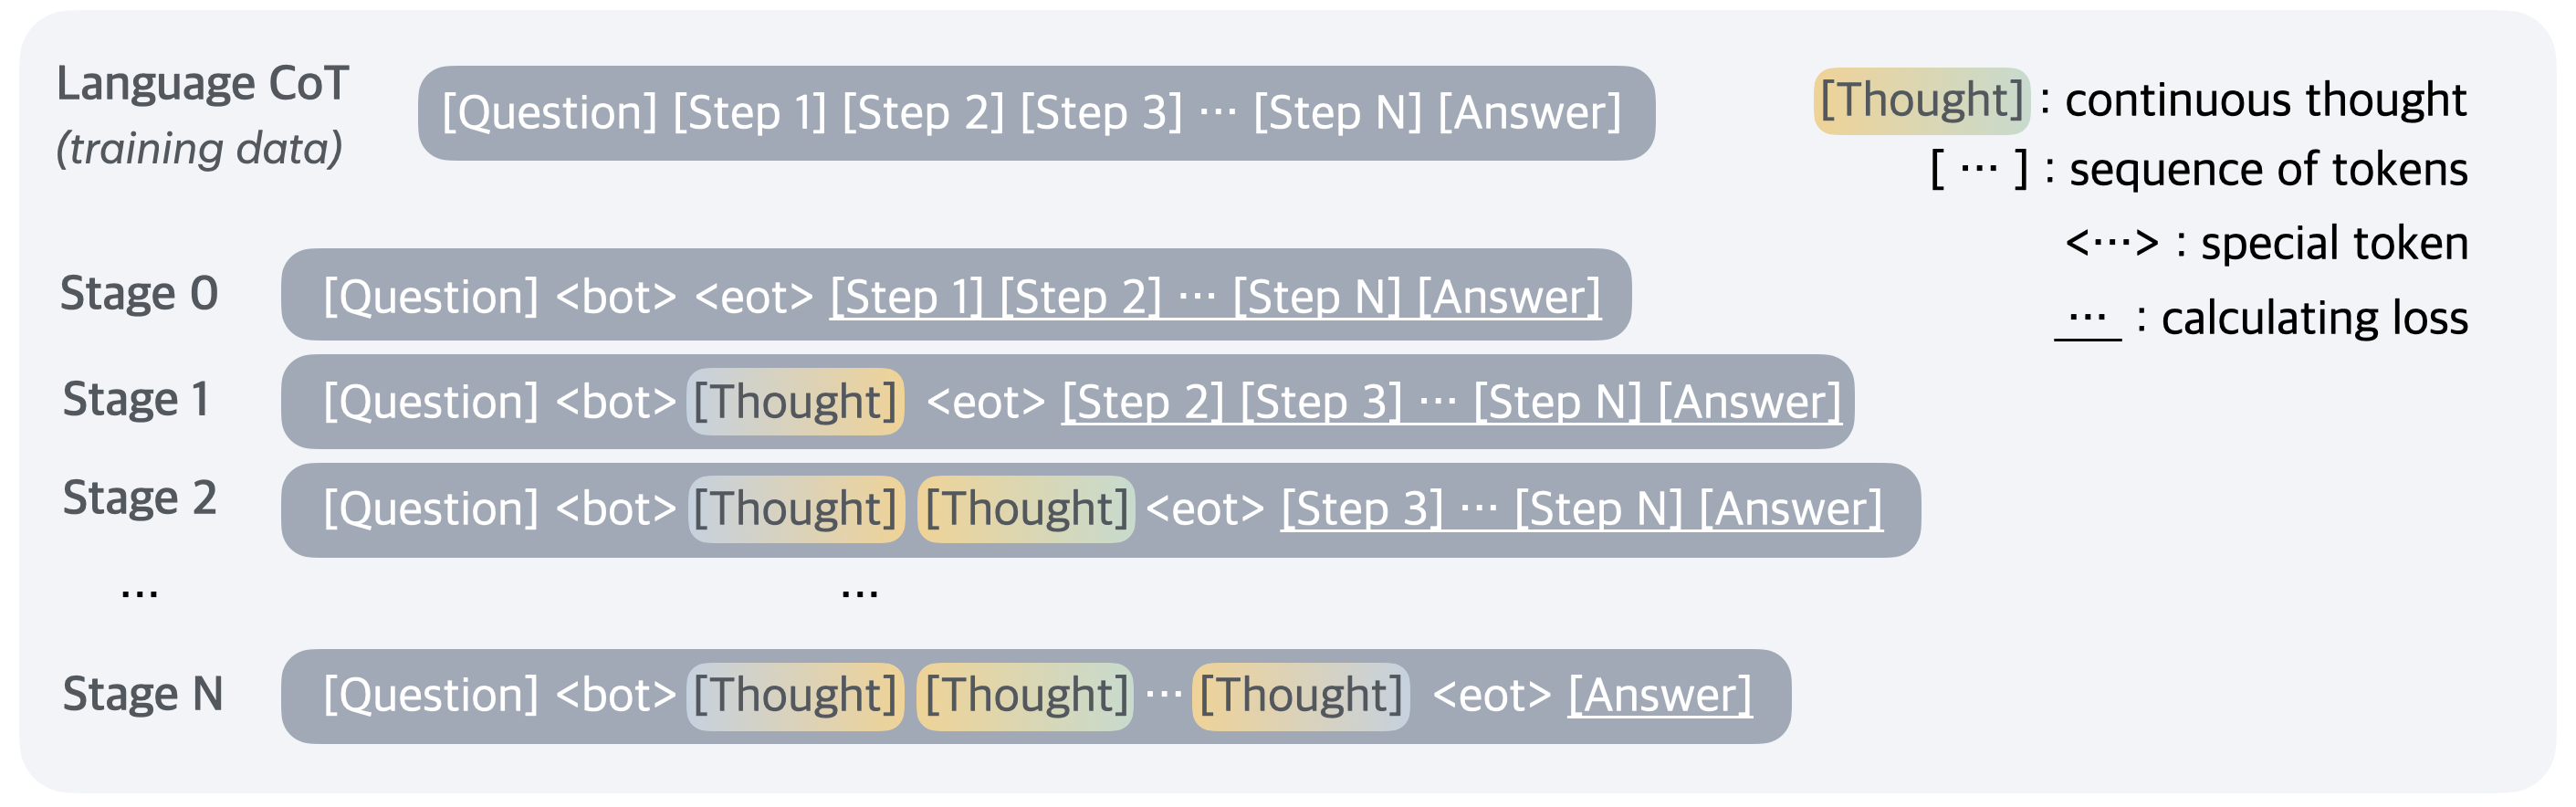
\includegraphics[width=\linewidth]{figures/figure_2_meta_5.png}
    %\vspace{-10pt}
    \caption{Training procedure of Chain of Continuous Thought (\ours). 
    Given training data with language reasoning steps, at each training stage we integrate $c$ additional continuous thoughts ($c=1$ in this example), and remove one language reasoning step. The cross-entropy loss is then used on the remaining tokens after continuous thoughts.}
    \label{fig:training}
    %\vspace{-15pt}
\end{figure}

During the training process, we optimize the normal negative log-likelihood loss, but mask the loss on questions and latent thoughts. It is important to note that the objective does \textbf{not} encourage the continuous thought to \textit{compress the removed language thought}, but rather to \textit{facilitate the prediction of future reasoning}. Therefore, it's possible for the LLM to learn more effective representations of reasoning steps compared to human language. 

\textbf{Training Details.} Our proposed continuous thoughts are fully differentiable and allow for back-propagation. We perform $n+1$ forward passes when $n$ latent thoughts are scheduled in the current training stage, computing a new latent thought with each pass and finally conducting an additional forward pass to obtain a loss on the remaining text sequence. While we can save any repetitive computing by using a KV cache, the sequential nature of the multiple forward passes poses challenges for parallelism. Further optimizing the training efficiency of \ours remains an important direction for future research.


\noindent\textbf{Inference Process.} The inference process for \ours is analogous to standard language model decoding, except that in latent mode, we directly feed the last hidden state as the next input embedding. A challenge lies in determining when to switch between latent and language modes. As we focus on the problem-solving setting, we insert a \texttt{<bot>} token immediately following the question tokens. For \texttt{<eot>}, we consider two potential strategies: a) train a binary classifier on latent thoughts to enable the model to autonomously decide when to terminate the latent reasoning, or b) always pad the latent thoughts to a constant length. We found that both approaches work comparably well. Therefore, we use the second option in our experiment for simplicity, unless specified otherwise.


\section{Experiments}
\label{sec:experiment}
We validate the feasibility of LLM reasoning in a continuous latent space through experiments on three datasets. We mainly evaluate the accuracy by comparing the model-generated answers with the ground truth. The number of newly generated tokens per question is also analyzed, as a measure of reasoning efficiency. We report the clock-time comparison in Appendix~\ref{sec:clock}.


\subsection{Reasoning Tasks}

\label{sec:prosqa}

\noindent\textbf{Math Reasoning.}
We use GSM8k~\citep{cobbe2021training} as the dataset for math reasoning. It consists of grade school-level math problems. Compared to the other datasets in our experiments, the problems are more diverse and open-domain, closely resembling real-world use cases. Through this task, we explore the potential of latent reasoning in practical applications. To train the model, we use a synthetic dataset generated by~\citet{deng2023implicit}.

\noindent\textbf{Logical Reasoning.} Logical reasoning involves the proper application of known conditions to prove or disprove a conclusion using logical rules. This requires the model to choose from multiple possible reasoning paths, where the correct decision often relies on exploration and planning ahead.  We use 5-hop ProntoQA~\citep{saparov2022language} questions, with fictional concept names. 
%An example is shown in Figure~\ref{fig:motivation}. 
For each problem, a tree-structured ontology is randomly generated and described in natural language as a set of known conditions. The model is asked to judge whether a given statement is correct based on these conditions. This serves as a simplified simulation of more advanced reasoning tasks, such as automated theorem proving~\citep{chen2023theoremqa, alphaproof2024}.

We found that the generation process of ProntoQA could be more challenging, especially since the size of distracting branches in the ontology is always small, reducing the need for complex planning. To fix that, we apply a new dataset construction pipeline using randomly generated DAGs to structure the known conditions. The resulting dataset requires the model to perform substantial planning and searching over the graph to find the correct reasoning chain. We refer to this new dataset as ProsQA (\underline{Pro}of with \underline{S}earch \underline{Q}uestion-\underline{A}nswering). A visualized example is shown in Figure~\ref{fig:interpret}. More details of datasets can be found in Appendix~\ref{sec:dataset-appendix}.


\subsection{Experimental Setup}

We use a pre-trained GPT-2~\citep{radford2019language} as the base model for all experiments. The learning rate is set to $1\times 10^{-4}$ while the effective batch size is 128. Following \citet{deng2024explicit}, we also reset the optimizer when the training stages switch.

\noindent\textbf{Math Reasoning. }
By default, we use 2 latent thoughts (i.e., $c=2$) for each reasoning step. 
We analyze the correlation between performance and $c$ in Section~\ref{sec:result}. The model goes through 3 stages besides the initial stage. Then, we have an additional stage, where we still use $3\times c$ continuous thoughts as in the penultimate stage, but remove all the remaining language reasoning chain. This handles the long-tail distribution of reasoning chains longer than 3 steps. We train the model for 6 epochs in the initial stage, and 3 epochs in each remaining stage. 

\noindent\textbf{Logical Reasoning. }
We use one continuous thought for every reasoning step (i.e., $c=1$). The model goes through 6 training stages in addition to the initial stage, because the maximum number of reasoning steps is 6 in these two datasets. The model then fully reasons with continuous thoughts to solve the problems in the last stage. We train the model for 5 epochs per stage.

For all datasets, after the standard schedule, the model stays in the final training stage, until the 50th epoch. We select the checkpoint based on the accuracy on the validation set. For inference, we manually set the number of continuous thoughts to be consistent with their final training stage. We use greedy decoding for all experiments. 

\subsection{Baselines and Variants of \ours}
We consider the following baselines: (1) \textit{CoT}: We use the complete reasoning chains to train the language model with supervised finetuning, and during inference, the model generates a reasoning chain before outputting an answer. (2) \textit{No-CoT}: The LLM is trained to directly generate the answer without using a reasoning chain. (3) \textit{iCoT}~\citep{deng2024explicit}: The model is trained with language reasoning chains and follows a carefully designed schedule that ``internalizes'' CoT. As the training goes on, tokens at the beginning of the reasoning chain are gradually removed until only the answer remains. During inference, the model directly predicts the answer. (4) \textit{Pause token}~\citep{goyal2023think}: The model is trained using only the question and answer, without a reasoning chain. However, different from \textit{No-CoT}, special \texttt{<pause>} tokens are inserted between the question and answer, which are believed to provide the model with additional computational capacity to derive the answer. For a fair comparison, the number of \texttt{<pause>} tokens is set the same as continuous thoughts in \ours.


We also evaluate some variants of our method: (1) \textit{w/o curriculum}: Instead of the multi-stage training, we directly use the data from the last stage which only includes questions and answers to train \ours. The model uses continuous thoughts to solve the whole problem. (2) \textit{w/o thought}: We keep the multi-stage training which removes language reasoning steps gradually, but don't use any continuous latent thoughts. While this is similar to \textit{iCoT} in the high-level idea, the exact training schedule is set to be consistent with \ours, instead of \textit{iCoT}. This ensures a more strict comparison. (3) \textit{Pause as thought}: We use special \texttt{<pause>} tokens to replace the continuous thoughts, and apply the same multi-stage training curriculum as \ours.


\subsection{Results and Discussion}

\begin{table*}
    \centering
    \label{tab:main}
    %\small
    \vspace{-20pt}
    \begin{tabular}{@{}rcccccc}
    
    \toprule
    \multirow{2}{*}[-2pt]{Method} & \multicolumn{2}{c}{GSM8k} & \multicolumn{2}{c}{ProntoQA} & \multicolumn{2}{c}{\dataset}\\
    \cmidrule{2-7}
          & Acc. (\%) & \# Tokens & Acc. (\%) & \# Tokens & Acc. (\%) & \# Tokens \\
        \midrule
        % \cmidrule{1-8}
        CoT  & 42.9{\scriptsize$\ \pm$0.2} & 25.0 &  98.8{\scriptsize$\ \pm$0.8} & 92.5 &  77.5{\scriptsize$\ \pm$1.9} & 49.4 \\
        \midrule
        No-CoT  & 16.5{\scriptsize$\ \pm$0.5} & 2.2 & 93.8{\scriptsize$\ \pm$0.7}  & 3.0 & 76.7{\scriptsize$\ \pm$1.0} & 8.2 \\
        iCoT  & 30.0$^*$ &  2.2 &  99.8{\scriptsize$\ \pm$0.3} &  3.0 & 98.2{\scriptsize$\ \pm$0.3} & 8.2 \\
        Pause Token &  16.4{\scriptsize$\ \pm$1.8} & 2.2 & 77.7{\scriptsize$\ \pm$21.0} & 3.0 &  75.9{\scriptsize$\ \pm$0.7} & 8.2 \\
        % \midrule
        %ROSCOE & 0.60 & - & - & 0.57 & 0.79 & - & - \\
        \midrule
        
        \ours (Ours) & 34.1{\scriptsize$\ \pm$1.5} & 8.2  & 99.8{\scriptsize$\ \pm$0.2} & 9.0 &  97.0{\scriptsize$\ \pm$0.3} & 14.2 \\
        
        - \textit{w/o curriculum} & 14.4{\scriptsize$\ \pm$0.8} & 8.2 & 52.4{\scriptsize$\ \pm$0.4} & 9.0 &  76.1{\scriptsize$\ \pm$0.2} & 14.2 \\
        - \textit{w/o thought} & 21.6{\scriptsize$\ \pm$0.5}  & 2.3 &  99.9{\scriptsize$\ \pm$0.1} & 3.0 &  95.5{\scriptsize$\ \pm$1.1} & 8.2 \\
        - \textit {pause as thought} & 24.1{\scriptsize$\ \pm$0.7} & 2.2 & 100.0{\scriptsize$\ \pm$0.1} & 3.0 &  96.6{\scriptsize$\ \pm$0.8} & 8.2 \\
        % \midrule
    \bottomrule 
    \end{tabular}
    %%
     \small
    %\vspace{-5pt}
    \caption{Results on three datasets: GSM8l, ProntoQA and ProsQA. Higher accuracy indicates stronger reasoning ability, while generating fewer tokens indicates better efficiency. $^*$The result is from \citet{deng2024explicit}.}
    \label{tab:main}
    \vspace{-10pt}
\end{table*}


\label{sec:result}

\begin{wrapfigure}{r}{0.4\linewidth}
    \centering
    \vspace{-15pt}
    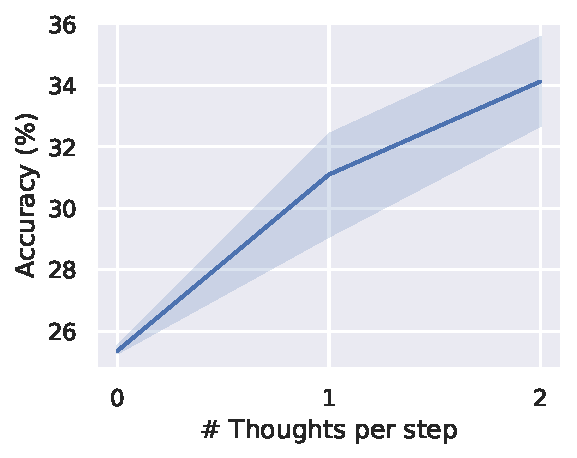
\includegraphics[width=\linewidth]{figures/n_latent.pdf}
    \vspace{-10pt}
    \caption{Accuracy on GSM8k with different number of continuous thoughts.}
    \vspace{-5pt}
    \label{fig:n_thoughts}
\end{wrapfigure}
We show the overall results on all datasets in Table~\ref{tab:main}. Continuous thoughts effectively enhance LLM reasoning, as shown by the consistent improvement over \textit{no-CoT}. It even shows better performance than \textit{CoT} on ProntoQA and ProsQA. We describe several key conclusions from the experiments as follows.



\noindent \textbf{``Chaining'' continuous thoughts enhances reasoning.} In conventional CoT, the output token serves as the next input, which proves to increase the effective depth of LLMs and enhance their expressiveness~\citep{feng2023towards}. We explore whether latent space reasoning retains this property, as it would suggest that this method could scale to solve increasingly complex problems by chaining multiple latent thoughts.

In our experiments with GSM8k, we found that \ours outperformed other architectures trained with similar strategies, particularly surpassing the latest baseline, \textit{iCoT}~\citep{deng2024explicit}. The performance is significantly better than \ours (\textit{pause as thought}) which also enables more computation in the LLMs.  While \cite{pfau2024let} empirically shows that filler tokens, such as the special \texttt{<pause>} tokens, can benefit highly parallelizable problems, our results show that \ours architecture is more effective for general problems, e.g., math word problems, where a reasoning step often heavily depends on previous steps. Additionally, we experimented with adjusting the hyperparameter $c$, which controls the number of latent thoughts corresponding to one language reasoning step (Figure~\ref{fig:n_thoughts}). As we increased $c$ from 0 to 1 to 2, the model’s performance steadily improved.\footnote{We discuss the case of larger $c$ in Appendix~\ref{sec:larger_c}.} These results suggest that a chaining effect similar to CoT can be observed in the latent space.

In two other synthetic tasks, we found that the variants of \ours (\textit{w/o thoughts} or \textit{pause as thought}), and the \textit{iCoT} baseline also achieve impressive accuracy. This indicates that the model’s computational capacity may not be the bottleneck in these tasks. In contrast, GSM8k, being an open-domain question-answering task, likely involves more complex contextual understanding and modeling, placing higher demands on computational capability. 

\noindent \textbf{Latent reasoning outperforms language reasoning in planning-intensive tasks.} 
Complex reasoning often requires the model to ``look ahead'' and evaluate the appropriateness of each step. Among our datasets, GSM8k and ProntoQA are relatively straightforward for next-step prediction, due to intuitive problem structures and limited branching. In contrast, ProsQA’s randomly generated DAG structure significantly challenges the model’s planning capabilities. As shown in Table~\ref{tab:main}, \textit{CoT} does not offer notable improvement over \textit{No-CoT}. However, \ours, its variants, and \textit{iCoT} substantially enhance reasoning on ProsQA, indicating that latent space reasoning provides a clear advantage in tasks demanding extensive planning. An in-depth analysis of this process is provided in Section~\ref{sec:understanding}.


\noindent \textbf{The LLM still needs guidance to learn latent reasoning.} 
In the ideal case, the model should learn the most effective continuous thoughts automatically through gradient descent on questions and answers (i.e., \ours \textit{w/o curriculum}). However, from the experimental results, we found  the models trained this way do not perform any better than no-CoT.



\begin{wrapfigure}{r}{0.48\linewidth}
    \centering
    \vspace{-10pt}
    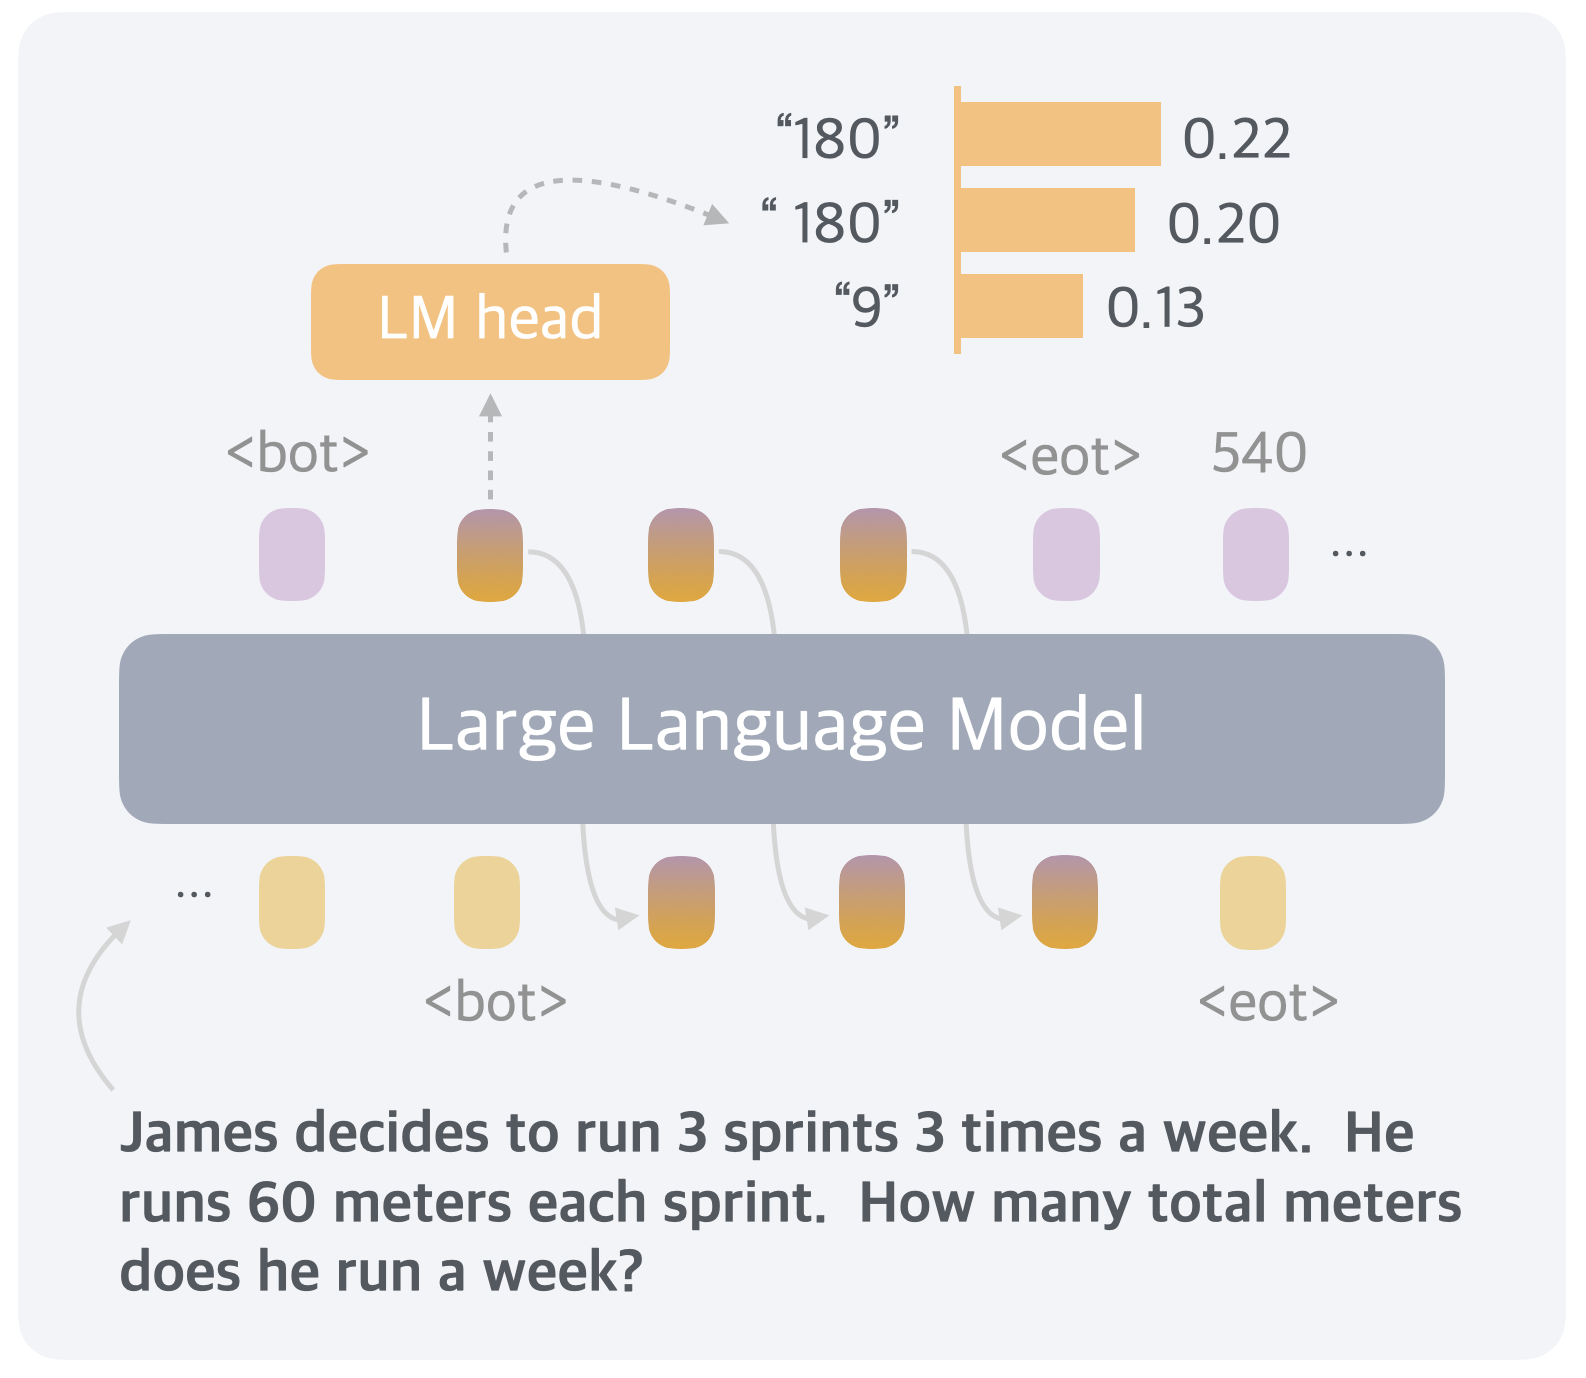
\includegraphics[width=\linewidth]{figures/figure_4_meta.png}
    \caption{A case study where we decode the continuous thought into language tokens.}
    \vspace{-10pt}
    \label{fig:case}
\end{wrapfigure}

With the multi-stage curriculum which decomposes the training into easier objectives, \ours is able to achieve top performance across various tasks. The multi-stage training also integrates well with pause tokens (\ours - \textit{pause as thought}). Despite using the same architecture and similar multi-stage training objectives, we observed a small gap between the performance of \textit{iCoT} and \ours (\textit{w/o thoughts}). The finer-grained removal schedule (token by token) and a few other tricks in \textit{iCoT} may ease the training process. We leave combining \textit{iCoT} and \ours as future work. While the multi-stage training used for \ours has proven effective, further research is definitely needed to develop better and more general strategies for learning reasoning in latent space, especially without the supervision from language reasoning chains.


\noindent \textbf{Continuous thoughts are efficient representations of reasoning.} 
Though the continuous thoughts are not intended to be decoded to language tokens, we can still use it as an intuitive interpretation of the continuous thought. We show a case study in Figure~\ref{fig:case} of a math word problem solved by \ours ($c=1$). The first continuous thought can be decoded into tokens like ``180'', `` 180'' (with a space), and ``9''. Note that, the reasoning trace for this problem should be $3\times 3 \times 60 = 9 \times 60 = 540$, or  $3\times 3 \times 60 = 3 \times 180 = 540$. The interpretations of the first thought happen to be the first intermediate variables in the calculation. Moreover, it encodes a distribution of different traces into the continuous thoughts. As shown in Section~\ref{sec:interpret}, this feature enables a more advanced reasoning pattern for planning-intense reasoning tasks.

% \begin{table*}[t]
%     \centering
%     \begin{NiceTabular}{lcccccc}
%     \CodeBefore
%     \rectanglecolor{metabg}{3-4}{4-4}
%     \rectanglecolor{metabg}{5-6}{6-6}
%     \Body
%     \toprule
%                                &   & \multicolumn{3}{c}{Vision tasks} & \multicolumn{2}{c}{Language tasks}\\
%     \cmidrule{3-7}
%                                &               & DatasetA             & DatasetB             & DatasetC             & DatasetD             & DatasetE \\
%     \midrule
%     \multirow{2}{*}{BaselineA} & $\lambda = 0$ & $\nm{0.84 \pm 0.22}$ & $\bm{0.83 \pm 0.14}$ & $\nm{0.84 \pm 0.24}$ & $\nm{0.86 \pm 0.16}$ & $\nm{0.81 \pm 0.18}$\\
%                                & $\lambda = 1$ & $\nm{0.83 \pm 0.26}$ & $\nm{0.82 \pm 0.20}$ & $\nm{0.88 \pm 0.23}$ & $\nm{0.87 \pm 0.12}$ & $\nm{0.84 \pm 0.20}$\\
%     \multirow{2}{*}{BaselineB} & $\lambda = 0$ & $\nm{0.84 \pm 0.15}$ & $\nm{0.86 \pm 0.16}$ & $\nm{0.89 \pm 0.11}$ & $\nm{0.84 \pm 0.17}$ & $\nm{0.87 \pm 0.30}$\\
%                                & $\lambda = 1$ & $\bm{0.90 \pm 0.15}$ & $\nm{0.81 \pm 0.22}$ & $\nm{0.88 \pm 0.18}$ & $\nm{0.83 \pm 0.23}$ & $\nm{0.80 \pm 0.27}$\\
%     \midrule 
%     \textbf{Our method}        &               & $\nm{0.86 \pm 0.19}$ & $\nm{0.81 \pm 0.18}$ & $\bm{0.95 \pm 0.16}$ & $\bm{0.91 \pm 0.13}$ & $\bm{0.92 \pm 0.30}$\\
%     \bottomrule
%     \end{NiceTabular}
%     \caption{A nice table does not require vertical separators and uses bolding---here implemented by the \texttt{\textbackslash{}bm\{\}} and \texttt{\textbackslash{}nm\{\}} commands---sparingly.
%     %
%     Using the \texttt{NiceTabular} environment from the \texttt{nicematrix} package to highlight the background of some cells easily, using the official \texttt{metabg} color.}
%     \label{table:demo}
% \end{table*}

% \lipsum[1-6]

% \begin{figure*}[t]
%      \centering
%      \begin{subfigure}[b]{0.48\textwidth}
%          \centering
%          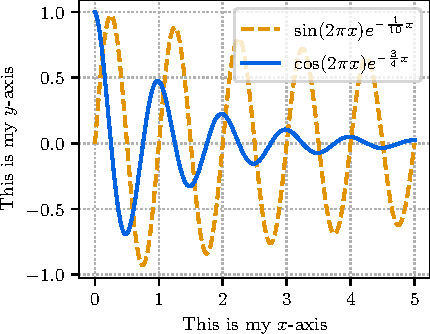
\includegraphics[]{assets/plot_demo.pdf}
%          \caption{First plot.}
%          \label{fig:plots:a}
%      \end{subfigure}
%      \hfill
%      \begin{subfigure}[b]{0.48\textwidth}
%          \centering
%          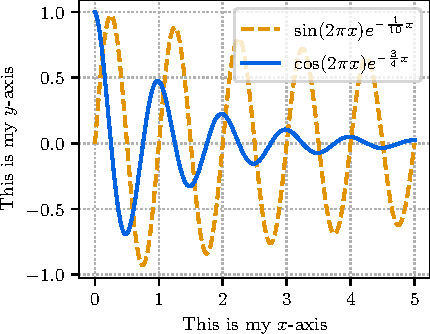
\includegraphics[]{assets/plot_demo.pdf}
%          \caption{Second plot.}
%          \label{fig:plots:b}
%      \end{subfigure}
%      \caption{Plots generated with the script \texttt{nice\_plot.py} included in this template.
%      % 
%      For more information on producing figures, please refer to \href{https://fb.workplace.com/notes/1767028093764250}{this Workplace post}.
%      %
%      If you would like to use a figure teaser, place it immediately after \texttt{\textbackslash{}maketitle}, forcing its location with the \texttt{[h!]} optional argument.
%      %
%      Please consider using the \href{https://www.facebook.com/brand/meta/color/}{Meta palette} to color your figures.
%      }
%      \label{fig:plots}
% \end{figure*}

% \lipsum[1-3]

\section{Understanding the Latent Reasoning in \ours}
\label{sec:understanding}
In this section, we present an analysis of the latent reasoning process with a variant of \ours. 
By leveraging its ability to switch between language and latent space reasoning, we are able to control the model to interpolate between fully latent reasoning and fully language reasoning and test their performance (Section~\ref{sec:understanding_results}). This also enables us to interpret the the latent reasoning process as tree search (Section~\ref{sec:interpret}). Based on this perspective, we explain why latent reasoning can make the decision easier for LLMs (Section~\ref{sec:height}).


%This is especially helpful to understand why \ours and some other latent reasoning methods can outperform CoT on ProsQA while generating much fewer tokens. 

% We study the performance of the \ours model while interpolating between fully latent reasoning and fully language reasoning (Section~\ref{sec:understanding_results}), and 



\subsection{Experimental Setup}
\label{sec:search_setup}
\noindent\textbf{Methods.} 
%In our default setting, \ours may . Specifically, we can control the placement of \texttt{<eot>} to determine the number of latent thoughts. For example, if we place \texttt{<eot>} after one latent thought, the model should generate the remaining language reasoning chain from the second step onwards. 
The design of \ours allows us to control the number of latent thoughts by manually setting the position of the \texttt{<eot>} token during inference. When we enforce \ours to use $k$ continuous thoughts, the model is expected to output the remaining reasoning chain in language, starting from the $k+1$ step. In our experiments, we test variants of \ours on ProsQA with $k \in \{0, 1, 2, 3, 4, 5, 6\}$. Note that all these variants only differ in inference time while sharing the same model weights. Besides, we report the performance of \textit{CoT} and \textit{no-CoT} as references. 

To address the issue of forgetting earlier training stages, we modify the original multi-stage training curriculum by always mixing data from other stages with a certain probability ($p=0.3$). This updated training curriculum yields similar performance and enables effective control over the switch between latent and language reasoning.

\noindent\textbf{Metrics.} We apply two sets of evaluation metrics. One of them is based on the correctness of the \textit{final answer}, regardless of the reasoning process. It is the metric used in the main experimental results above (Section~\ref{sec:result}). To enable fine-grained analysis, we define another metric on the \textit{reasoning process}. Assuming we have a complete language reasoning chain which specifies a path in the graph, we can classify it into (1) \textbf{Correct Path}: The output is one of the shortest paths to the correct answer. (2) \textbf{Longer Path}: A valid path that correctly answers the question but is longer than the shortest path. (3) \textbf{Hallucination}: The path includes nonexistent edges or is disconnected. (4) \textbf{Wrong Target}: A valid path in the graph, but the destination node is not the one being asked. These four categories naturally apply to the output from  \ours ($k=0$) and \textit{CoT}, which generate the full path. For \ours with $k>0$ that outputs only partial paths in language (with the initial steps in continuous reasoning), we classify the reasoning as a Correct Path \textit{if a valid explanation can complete it}. Also, we define Longer Path and Wrong Target for partial paths similarly. If no valid explanation completes the path, it’s classified as hallucination. In \textit{no-CoT} and \ours with larger $k$, the model may only output the final answer without any partial path, and it falls into (5) \textbf{Correct Label} or (6) \textbf{Incorrect Label}. These six categories cover all cases without overlap.

\begin{figure}
    \centering
    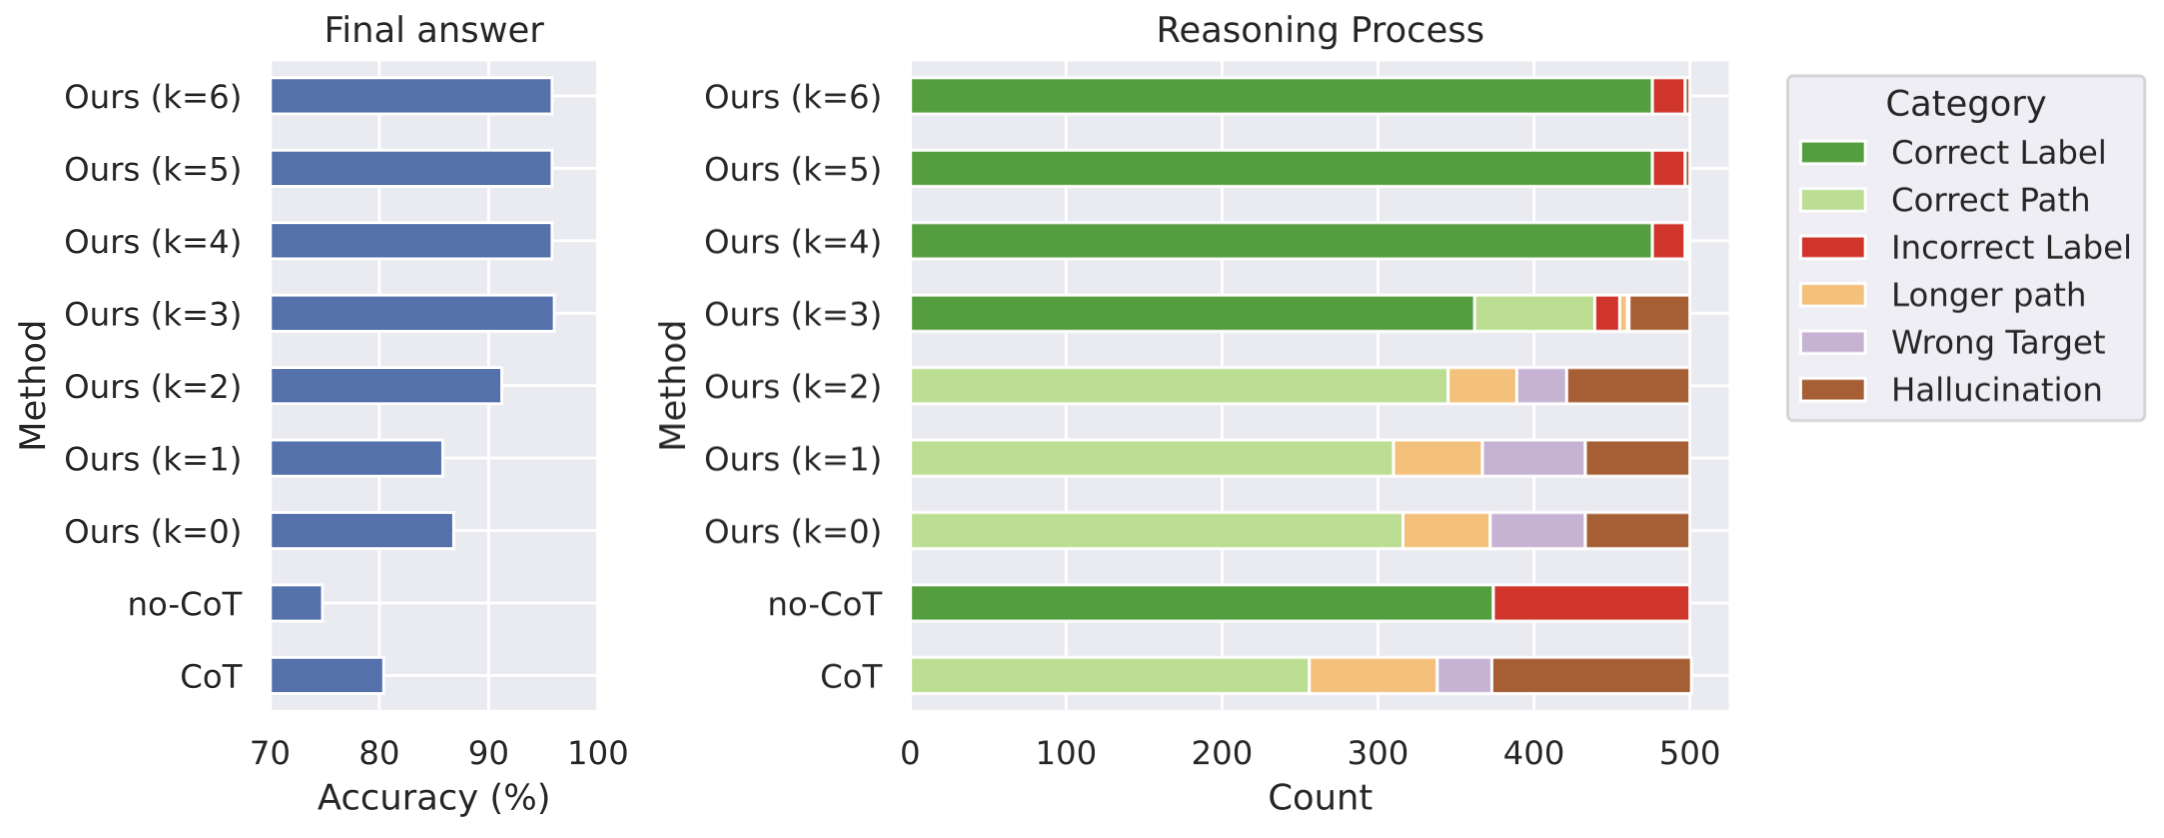
\includegraphics[width=\linewidth]{figures/figure_5_revised_1111.png}
    \caption{The accuracy of final answer (left) and reasoning process (right) of multiple variants of \ours and baselines on ProsQA.}
    \label{fig:analysis}
\end{figure}


\begin{figure}[H]
    \centering
    \vspace{-15pt}
    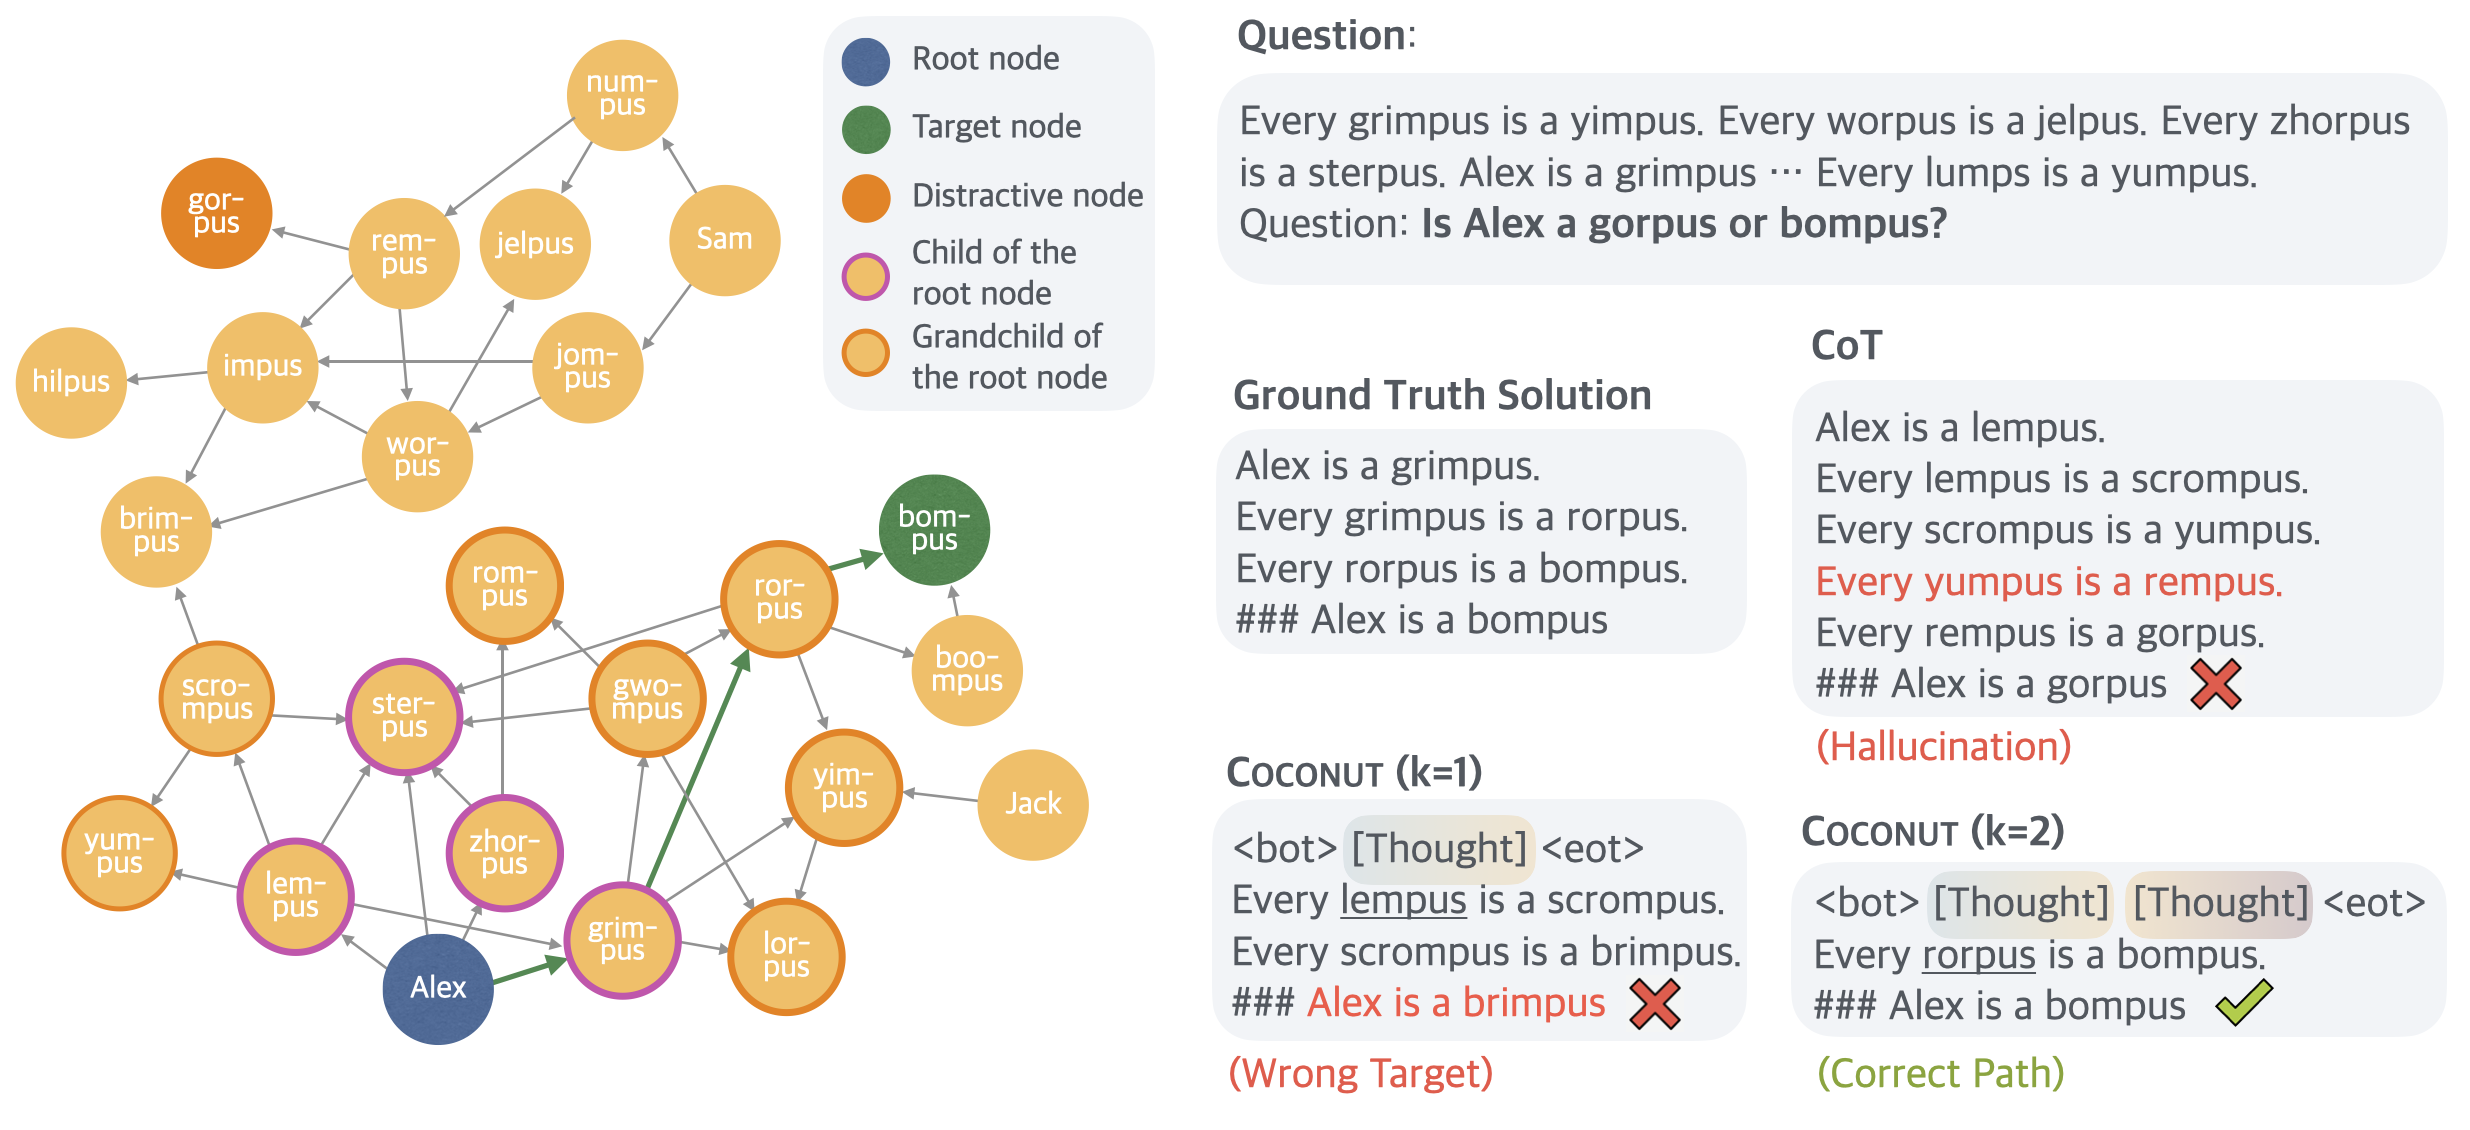
\includegraphics[width=1\linewidth]{figures/figure_6_meta_3.png}
    
    %\vspace{-10pt}
    \caption{A case study of ProsQA. The model trained with \textit{CoT} hallucinates an edge (\textit{Every yumpus is a rempus}) after getting stuck in a dead end. \ours (k=1) outputs a path that ends with an irrelevant node. \ours (k=2) solves the problem correctly.
    %The height (h) of a node is defined as the longest distance to any leaf nodes.
    }
    \label{fig:interpret}
    %\vspace{-5pt}
    \centering
    
    \vspace{15pt}
    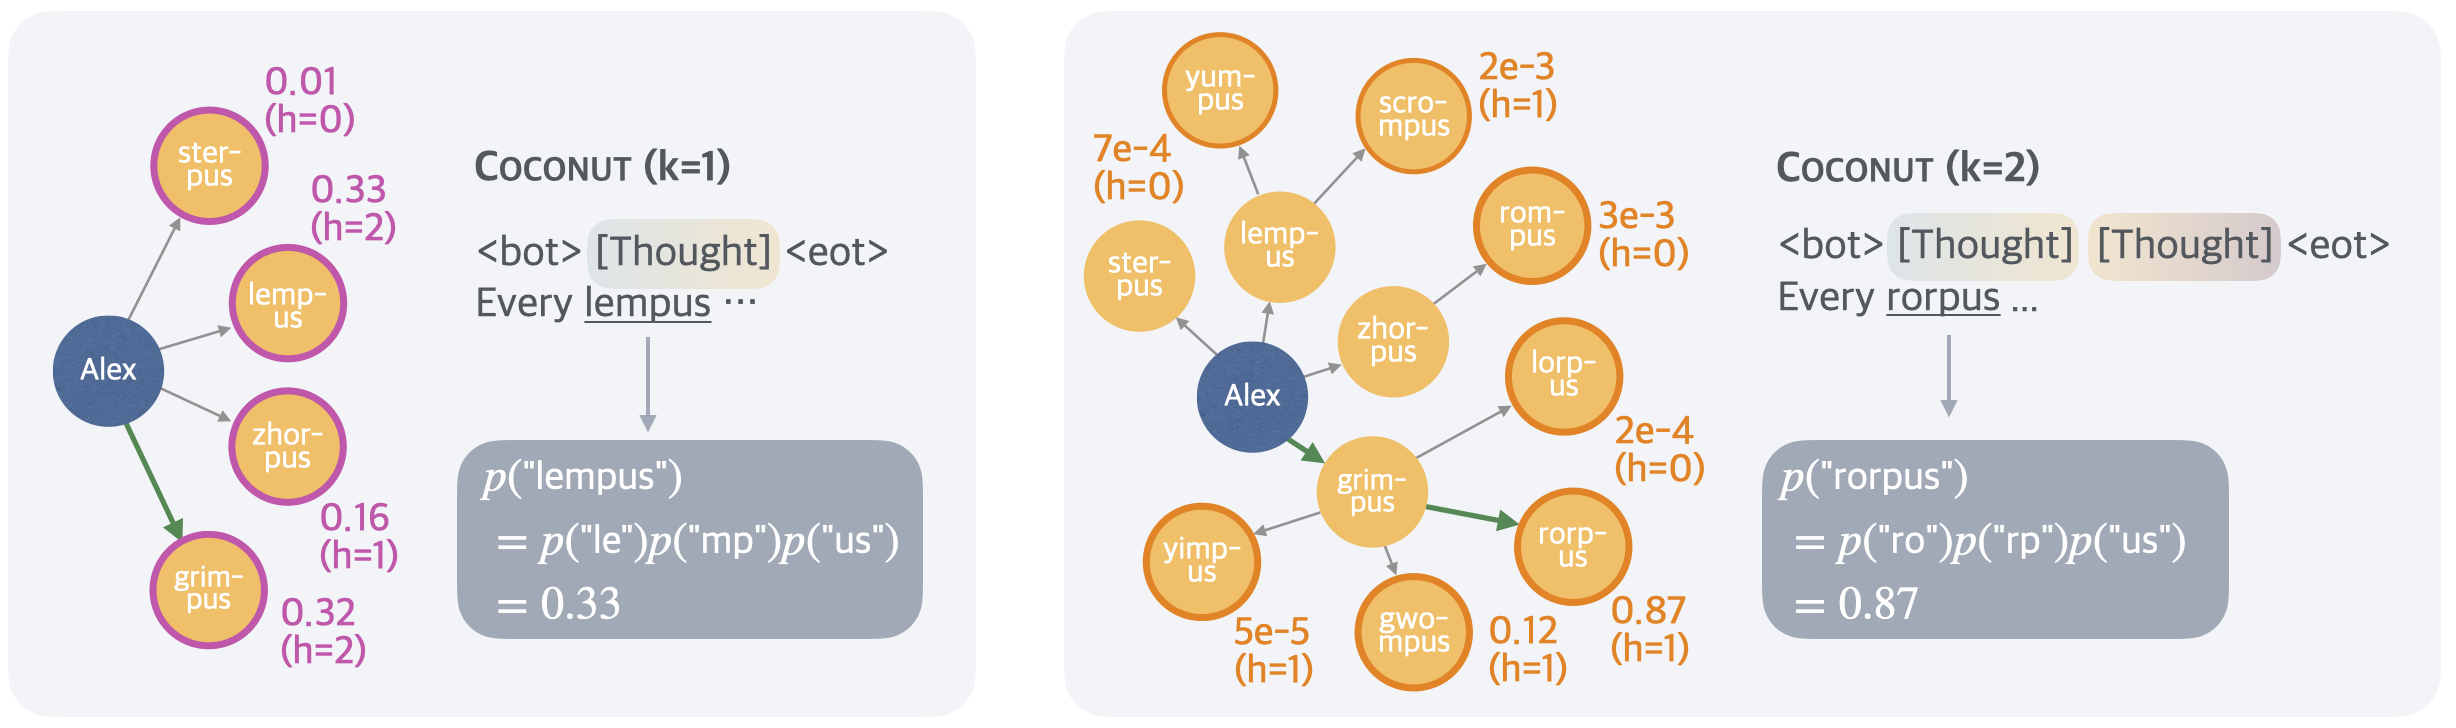
\includegraphics[width=\linewidth]{figures/figure_7_meta_4.png}
    
    %\vspace{-5pt}
    \caption{An illustration of the latent search trees. The example is the same test case as in Figure~\ref{fig:interpret}. The height of a node (denoted as $h$ in the figure) is defined as the longest distance to any leaf nodes in the graph. We show the probability of the first concept predicted by the model following latent thoughts (e.g., ``lempus'' in the left figure). It is calculated as the multiplication of the probability of all tokens within the concept conditioned on previous context (omitted in the figure for brevity). This metric can be interpreted as an implicit value function estimated by the model, assessing the potential of each node leading to the correct answer.}
    \label{fig:height}
    \vspace{-10pt}
\end{figure}

\subsection{Interpolating between Latent and Language Reasoning}

\label{sec:understanding_results}


Figure~\ref{fig:analysis} shows a comparative analysis of different reasoning methods on ProsQA. As more reasoning is done with continuous thoughts (increasing $k$), both final answer accuracy (Figure~\ref{fig:analysis}, left) and the rate of correct reasoning processes (``Correct Label'' and ``Correct Path'' in Figure~\ref{fig:analysis}, right) improve. Additionally, the rate of ``Hallucination'' and ``Wrong Target'' decrease, which typically occur when the model makes a wrong move earlier. This also indicates the better planning ability when more reasoning happens in the latent space.

A case study is shown in Figure~\ref{fig:interpret}, where \textit{CoT} hallucinates an nonexistent edge, \ours ($k=1$) leads to a wrong target, but \ours ($k=2$) successfully solves the problem. In this example, the model cannot accurately determine which edge to choose at the earlier step. However, as latent reasoning can avoid making a hard choice upfront, the model can progressively eliminate incorrect options in subsequent steps and achieves higher accuracy at the end of reasoning. We show more evidence and details of this reasoning process in Section~\ref{sec:interpret}. 


The comparison between \textit{CoT} and \ours ($k=0$) reveals another interesting observation: even when \ours is forced to generate a complete reasoning chain, the accuracy of the answers is still higher than \textit{CoT}. The generated reasoning paths are also more accurate with less hallucination. From this, we can infer that the training method of mixing different stages improves the model's ability to plan ahead. The training objective of \textit{CoT} always concentrates on the generation of the immediate next step, making the model ``shortsighted''. In later stages of \ours training, the first few steps are hidden, allowing the model to focus more on future steps. This is related to the findings of \citet{gloeckle2024better}, where they propose multi-token prediction as a new pretraining objective to improve the LLM's ability to plan ahead.



\subsection{Interpreting the Latent Search Tree}
\label{sec:interpret}



Given the intuition that continuous thoughts can encode multiple potential next steps, the latent reasoning can be interpreted as a search tree, rather than merely a reasoning ``chain''. Taking the case of Figure~\ref{fig:interpret} as a concrete example, the first step could be selecting one of the children of \textit{Alex}, i.e., \textit{\{lempus, sterpus, zhorpus, grimpus\}}. We depict all possible branches in the left part of Figure~\ref{fig:height}. Similarly, in the second step, the frontier nodes will be the grandchildren of \textit{Alex} (Figure~\ref{fig:height}, right). 


Unlike a standard breadth-first search (BFS), which explores all frontier nodes uniformly, the model demonstrates the ability to prioritize promising nodes while pruning less relevant ones. To uncover the model's preferences, we analyze its subsequent outputs in language space. For instance, if the model is forced to switch back to language space after a single latent thought ($k=1$), it predicts the next step in a structured format, such as ``every [Concept A] is a [Concept B].'' By examining the probability distribution over potential fillers for [Concept A], we can derive numeric values for the children of the root node \textit{Alex} (Figure~\ref{fig:height}, left). Similarly, when $k=2$, the prediction probabilities for all frontier nodes—the grandchildren of \textit{Alex}—are obtained (Figure~\ref{fig:height}, right).


\begin{figure}
    \centering
    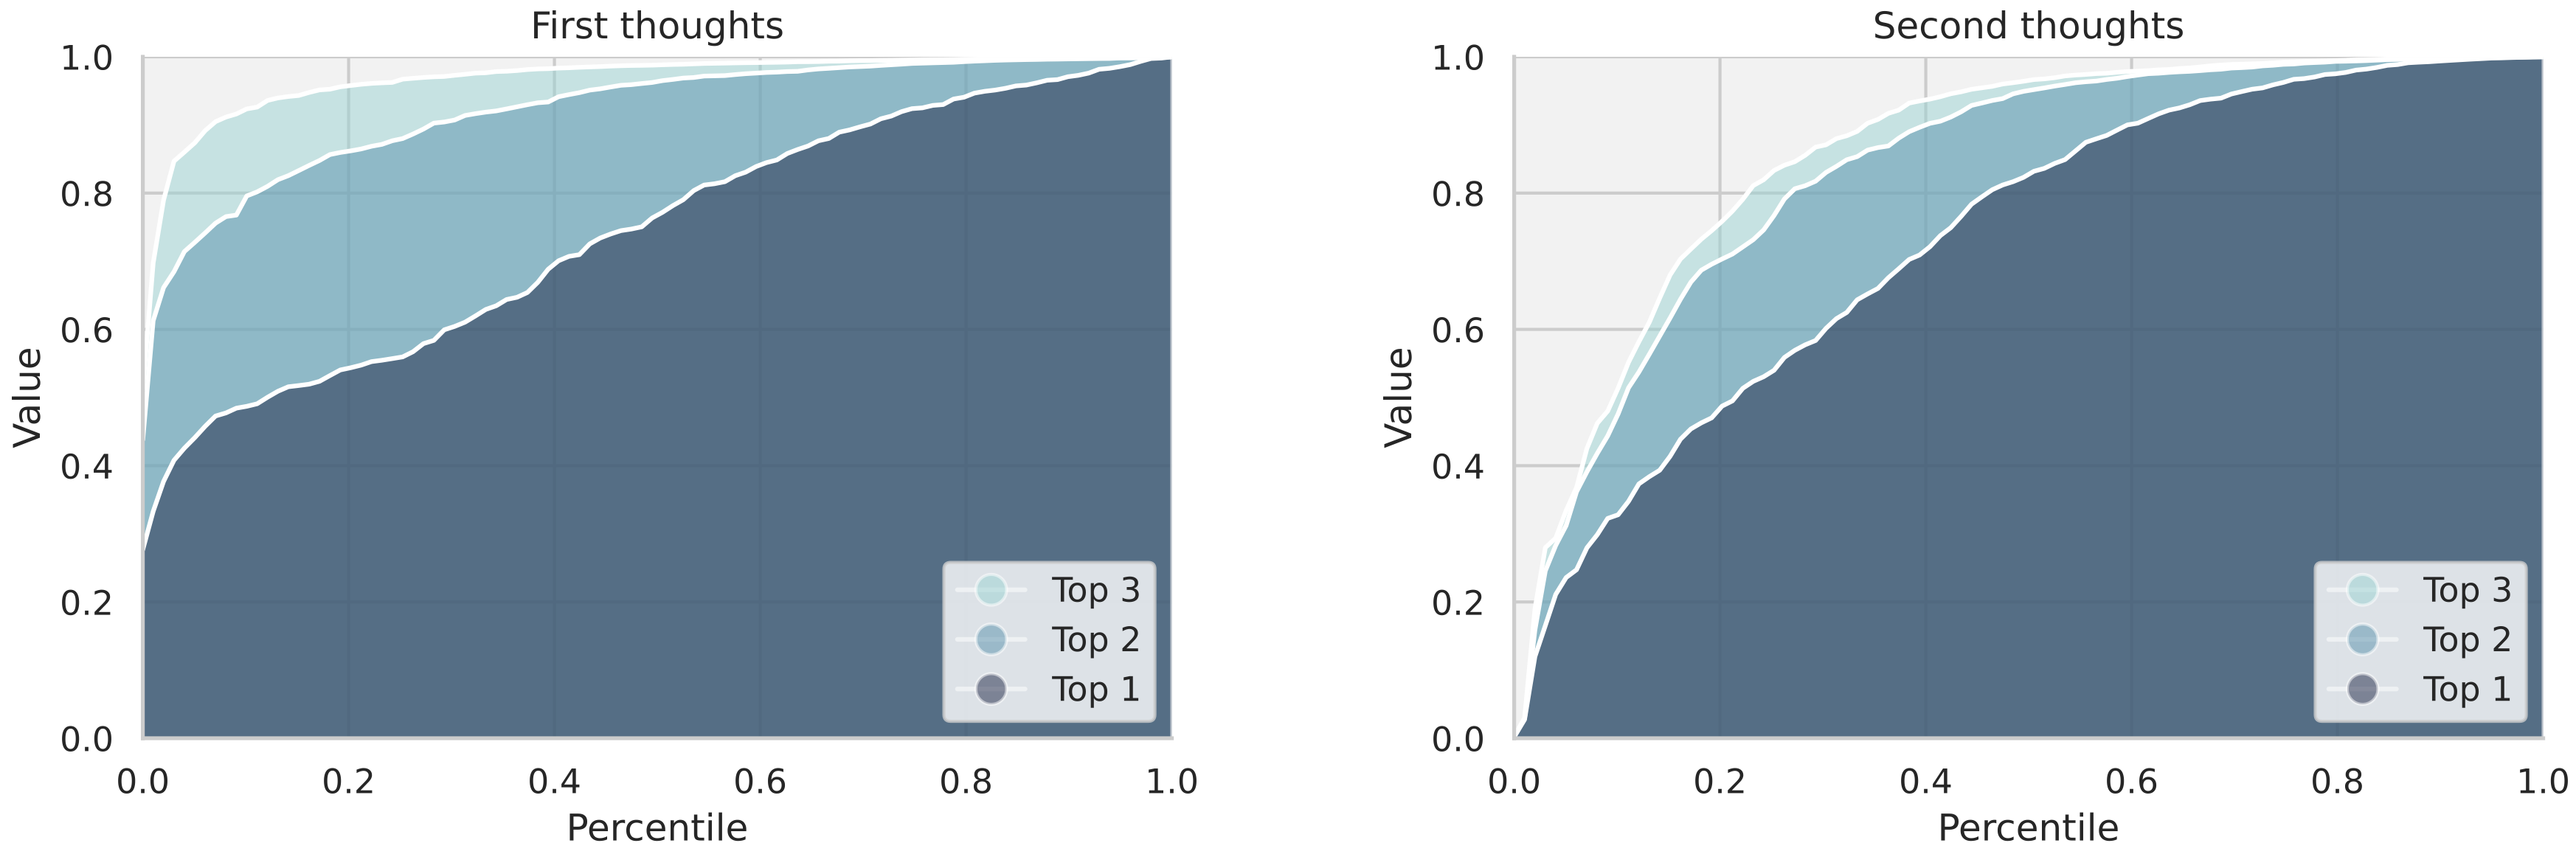
\includegraphics[width=\linewidth]{figures/percentile.png}
    %\vspace{-5pt}
    \caption{Analysis of parallelism in latent tree search. The left plot depicts the cumulative value of the top-1, top-2, and top-3 candidate nodes for the first thoughts, calculated across test cases and ranked by percentile. The significant gaps between the lines reflect the model's ability to explore alternative latent thoughts in parallel. The right plot shows the corresponding analysis for the second thoughts, where the gaps between lines are narrower, indicating reduced parallelism and increased certainty in reasoning as the search tree develops. This shift highlights the model's transition toward more focused exploration in later stages.}
    \label{fig:percentile}
    %\vspace{-5pt}
\end{figure}

The probability distribution can be viewed as the model's implicit \textit{value function}, estimating each node's potential to reach the target. As shown in the figure, ``lempus'', ``zhorpus'', ``grimpus'', and ``sterpus'' have a value of 0.33, 0.16, 0.32, and 0.01, respectively. This indicates that in the first continuous thought, the model has mostly ruled out ``sterpus'' as an option but remains uncertain about the correct choice among the other three. In the second thought, however, the model has mostly ruled out other options but focused on ``rorpus''.

Figure~\ref{fig:percentile} presents an analysis of the parallelism in the model's latent reasoning across the first and second thoughts. For the first thoughts (left panel), the cumulative values of the top-1, top-2, and top-3 candidate nodes are computed and plotted against their respective percentiles across the test set. The noticeable gaps between the three lines indicate that the model maintains significant diversity in its reasoning paths at this stage, suggesting a broad exploration of alternative possibilities. In contrast, the second thoughts (right panel) show a narrowing of these gaps. This trend suggests that the model transitions from parallel exploration to more focused reasoning in the second latent reasoning step, likely as it gains more certainty about the most promising paths. %This behavior highlights the model's ability to balance exploration and convergence as reasoning progresses.





\subsection{Why is a Latent Space Better for Planning?}
\label{sec:height}


\begin{wrapfigure}{r}{0.45\linewidth}
    \centering
    \vspace{-15pt}
    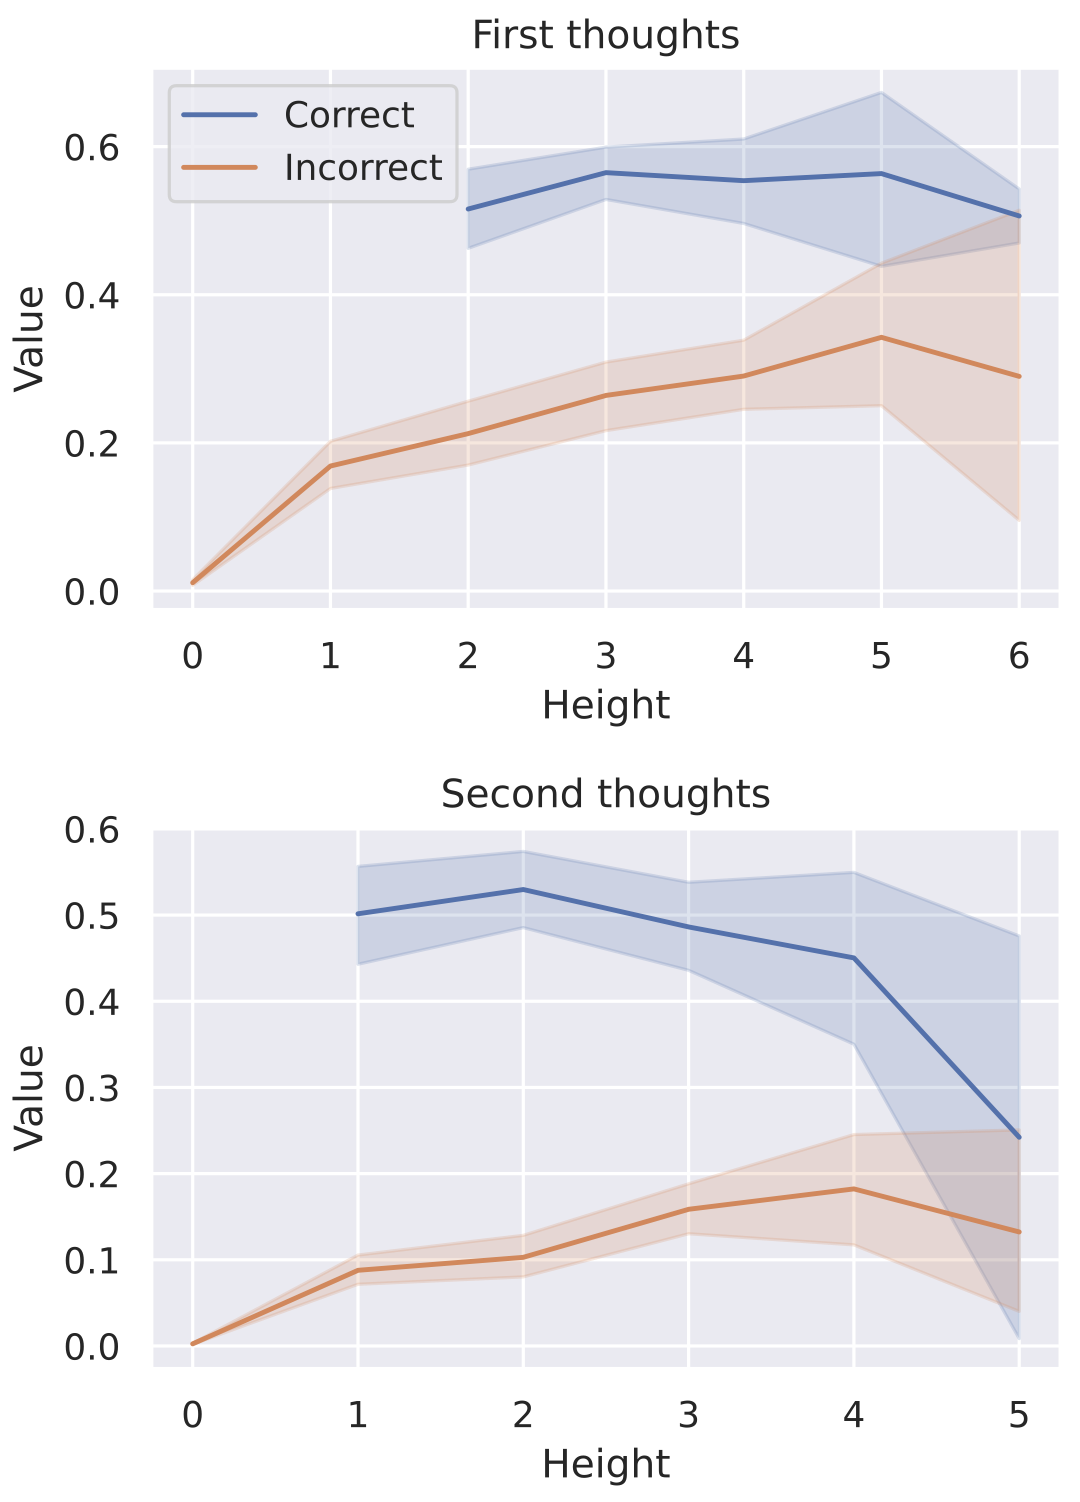
\includegraphics[width=\linewidth]{figures/value_stats_meta_2.png}
    \vspace{-15pt}
    \caption{The correlation between prediction probability of concepts and their heights.}
    \vspace{-15pt}
    \label{fig:height_pred}
\end{wrapfigure}

In this section, we explore why latent reasoning is advantageous for planning, drawing on the search tree perspective and the value function defined earlier. Referring to our illustrative example, a key distinction between \textit{``sterpus''} and the other three options lies in the structure of the search tree: \textit{``sterpus''} is a leaf node (Figure~\ref{fig:interpret}). This makes it immediately identifiable as an incorrect choice, as it cannot lead to the target node \textit{``bompus''}. In contrast, the other nodes have more descendants to explore, making their evaluation more challenging. 

To quantify a node's exploratory potential, we measure its height in the tree, defined as the shortest distance to any leaf node. Based on this notion, we hypothesize that \textit{nodes with lower heights are easier to evaluate accurately}, as their exploratory potential is limited. Consistent with this hypothesis, in our example, the model exhibits greater uncertainty between \textit{``grimpus''} and \textit{``lempus''}, both of which have a height of 2—higher than the other candidates.


To test this hypothesis more rigorously, we analyze the correlation between the model’s prediction probabilities and node heights during the first and second latent reasoning steps across the test set. Figure~\ref{fig:height_pred} reveals a clear pattern: the model successfully assigns lower values to incorrect nodes and higher values to correct nodes when their heights are low. However, as node heights increase, this distinction becomes less pronounced, indicating greater difficulty in accurate evaluation.

In conclusion, these findings highlight the benefits of leveraging latent space for planning. By delaying definite decisions and expanding the latent reasoning process, the model pushes its exploration closer to the search tree’s terminal states, making it easier to distinguish correct nodes from incorrect ones.

\section{Conclusion}

In this paper, we presented \ours, a novel paradigm for reasoning in continuous latent space. Through extensive experiments, we demonstrated that \ours significantly enhances LLM reasoning capabilities. Notably, our detailed analysis highlighted how an unconstrained latent space allows the model to develop an effective reasoning pattern similar to BFS. Future work is needed to further refine and scale latent reasoning methods. One promising direction is pretraining LLMs with continuous thoughts, which may enable models to generalize more effectively across a wider range of reasoning scenarios. We anticipate that our findings will inspire further research into latent reasoning methods, ultimately contributing to the development of more advanced machine reasoning systems.


%\section{Acknowledgement}
\newpage
{\Large \sffamily Acknowledgement\par}
The authors express their sincere gratitude to Jihoon Tack for his valuable discussions throughout the course of this work.


\bibliographystyle{assets/plainnat}
\bibliography{paper}

\clearpage
\newpage
\beginappendix
\section{Datasets}
\label{sec:dataset-appendix}

\subsection{Examples}
We provide some examples of the questions and CoT solutions for the datasets used in our experiments.

\begin{tcolorbox}[title=GSM8k, colback=white]
\texttt{Question = "John cuts his grass to 2 inches.  It grows .5 inches per month.  When it gets to 4 inches he cuts it back down to 2 inches.  It cost \$100 to get his grass cut.  How much does he pay per year?" \\ Steps = ["<<4-2=2>>", "<<2/.5=4>>", "<<12/4=3>>", "<<100*3=300>>"]\\
Answer = "300"
}
\end{tcolorbox}



\begin{tcolorbox}[title=ProntoQA, colback=white]
\texttt{Question = "Brimpuses are not luminous. Shumpuses are amenable. Each yumpus is a lorpus. Gorpuses are shumpuses. Each zumpus is a grimpus. Gorpuses are rompuses. Dumpuses are not floral. Lempuses are cold. Brimpuses are impuses. Every lorpus is floral. Every rompus is transparent. Grimpuses are muffled. Rompuses are yumpuses. Rompuses are wumpuses. Zumpuses are fast. Wumpuses are bitter. Every sterpus is orange. Each lorpus is a vumpus. Yumpuses are feisty. Each yumpus is a lempus. Gorpuses are snowy. Zumpuses are gorpuses. Every lorpus is a sterpus. Stella is a brimpus. Stella is a zumpus. True or false: Stella is not floral." \\ Steps = ["Stella is a zumpus. Zumpuses are gorpuses.", "Stella is a gorpus. Gorpuses are rompuses.", "Stella is a rompus. Rompuses are yumpuses.", "Stella is a yumpus. Each yumpus is a lorpus.", "Stella is a lorpus. Every lorpus is floral.", "Stella is floral."]\\
Answer = "False"
}
\end{tcolorbox}


\begin{tcolorbox}[title=ProsQA, colback=white]
\texttt{Question = "Every shumpus is a rempus. Every shumpus is a yimpus. Every terpus is a fompus. Every terpus is a gerpus. Every gerpus is a brimpus. Alex is a rempus. Every rorpus is a scrompus. Every rorpus is a yimpus. Every terpus is a brimpus. Every brimpus is a lempus. Tom is a terpus. Every shumpus is a timpus. Every yimpus is a boompus. Davis is a shumpus. Every gerpus is a lorpus. Davis is a fompus. Every shumpus is a boompus. Every shumpus is a rorpus. Every terpus is a lorpus. Every boompus is a timpus. Every fompus is a yerpus. Tom is a dumpus. Every rempus is a rorpus. Is Tom a lempus or scrompus?" \\ Steps = ["Tom is a terpus.", "Every terpus is a brimpus.", "Every brimpus is a lempus."]\\
Answer = "Tom is a lempus."
}
\end{tcolorbox}

\subsection{Construction of ProsQA}

To construct the dataset, we first compile a set of typical entity names, such as “Alex” and “Jack,” along with fictional concept names like “lorpus” and “rorpus,” following the setting of ProntoQA~\citep{saparov2022language}. Each problem is structured as a binary question: “Is [Entity] a [Concept A] or [Concept B]?” Assuming [Concept A] is the correct answer, we build a directed acyclic graph (DAG) where each node represents an entity or a concept. The graph is constructed such that a path exists from [Entity] to [Concept A] but not to [Concept B].

Algorithm~\ref{alg:prosqa} describes the graph construction process. The DAG is incrementally built by adding nodes and randomly connecting them with edges. To preserve the validity of the binary choice, with some probability, we enforce that the new node cannot simultaneously serve as a descendant to both node $0$ and $1$. This separation maintains distinct families of nodes and balances their sizes to prevent model shortcuts.

After the graph is constructed, nodes without parents are assigned entity names, while other nodes receive concept names. To formulate a question of the form “Is [Entity] a [Concept A] or [Concept B]?”, we designate node $0$ in the graph as [Entity], a leaf node labeled $1$ as [Concept A], and a leaf node labeled $2$ as [Concept B]. This setup ensures a path from [Entity] to [Concept A] without any connection to [Concept B], introducing a moderately complex reasoning path. Finally, to avoid positional biases, [Concept A] and [Concept B] are randomly permuted in each question.
% To construct the dataset, we need to a set of entities, which are typical names like ``Alex'', ``Jack'', etc, and a set of concepts, which are fictional words like ``lorpus'', ``rorpus'', etc. This follows the fictional setting of ProntoQA~\citep{saparov2022language}.

\begin{algorithm}
\caption{Graph Construction for ProsQA}\label{alg:prosqa}
\begin{algorithmic}

\State  $edges\gets \{\}$
\State  $nodes\gets \{0, 1\}$
\State  $labels\gets \{0: 1, 1:2\}$ \\ \Comment{Labels: 1 (descendant of node 0), 2 (descendant of node 1), 3 (both), 0 (neither).}
\State  $groups\gets \{0: \{\}, 1: \{0\}, 2:\{1\}, 3:\{\}\}$

\State $idx\gets 2$
\While{$idx < N$}

    \Comment{For each new node, randomly add edges from existing nodes}
    
    \State $n\_in\_nodes \gets \text{poisson}(1.5)$
    \State $rand \gets \text{random}()$

    \If{$rand \le 0.35$}
        \State $candidates \gets groups[0] \cup groups[1]$
        \Comment{Cannot be a descendant of node 1.}
    \ElsIf{$rand \le 0.7$}
        \State $candidates \gets groups[0] \cup groups[2]$
        \Comment{Cannot be a descendant of node 0.}
    \Else
        \State $candidates \gets nodes$
    \EndIf
    \State $n\_in\_nodes \gets \min(\text{len}(candidates), n\_in\_nodes)$
    \State $weights \gets [\text{depth\_to\_root}(c) \cdot 1.5 + 1 \;\forall c \in candidates]$ \\
    \Comment{Define sampling weights to prioritize deeper nodes.} \\
    \Comment{This way, the solution reasoning chain is expected to be longer.}

    \State $in\_nodes \gets \text{random\_choice}(candidates, n\_in\_nodes, \text{prob} = weights / \text{sum}(weights))$
    \State $cur\_label \gets 0$
    
    \For{$in\_idx \in in\_nodes$}
        \State $cur\_label \gets cur\_label \mid labels[in\_idx]$
        \Comment{Update label using bitwise OR.}
        \State $edges.\text{append}((in\_idx, idx))$
    \EndFor
    
    \State $groups[cur\_label].\text{append}(idx)$
    \State $labels[idx] \gets cur\_label$
    \State $nodes \gets nodes \cup \{idx\}$
    \State $idx \gets idx + 1$

\EndWhile
\end{algorithmic}
\end{algorithm}

\begin{table}[]

    \centering
    \begin{tabular}{c|c|c|c}
    \toprule
         \# Nodes & \# Edges & Len. of Shortest Path & \# Shortest Paths \\
         \midrule
           23.0 & 36.0 & 3.8 & 1.6 \\
          \bottomrule
    \end{tabular}
    \captionsetup{justification=centering}
    \caption{Statistics of the graph structure in ProsQA.}
    \label{tab:prosqa}
\end{table}

\subsection{Statistics}

We show the size of all datasets in Table~\ref{tab:stats}.

\begin{table}[]

    \centering
    \begin{tabular}{r|c|c|c}
    \toprule
         Dataset & Training & Validation & Test \\
         \midrule
           GSM8k & 385,620 & 500 & 1319 \\
           ProntoQA & 9,000 & 200 & 800 \\
           ProsQA & 17,886 & 300 & 500 \\
          \bottomrule
    \end{tabular}
    \captionsetup{justification=centering}
    \caption{Statistics of the datasets.}
    \label{tab:stats}
\end{table}


\section{Clock-Time Reasoning Efficiency Metric} \label{sec:clock}

We present a clock-time comparison to evaluate reasoning efficiency. The reported values represent the average inference time per test case (in seconds), with a batch size of 1, measured on an Nvidia A100 GPU. For the no-CoT and CoT baselines, we employ the standard generate method from the \texttt{transformers}\footnote{\url{https://github.com/huggingface/transformers}} library. Our results show that clock time is generally proportional to the number of newly generated tokens, as detailed in Table~\ref{tab:main}.



\begin{table}[h!]
    \centering
    \label{tab:efficiency}
    \begin{tabular}{lccc}
        \toprule
        Method & GSM8k & ProntoQA & ProsQA \\
        \midrule
        No-CoT & 0.03 & 0.03 & 0.08 \\
        CoT    & 0.26 & 0.85 & 0.47 \\
        \ours   & 0.09 & 0.11 & 0.15 \\
        \bottomrule
        
    \end{tabular}
    
    \captionsetup{justification=centering}
    \caption{Inference time (in seconds) comparison across tasks and methods.}
\end{table}

\section{Using More Continuous Thoughts}
\label{sec:larger_c}
In Figure~\ref{fig:n_thoughts}, we present the performance of \ours on GSM8k using $c \in \{0, 1, 2\}$. When experimenting with $c=3$, we observe a slight performance drop accompanied by increased variance. Analysis of the training logs indicates that adding three continuous thoughts at once -- particularly during the final stage transition -- leads to a sharp spike in training loss, causing instability. Future work will explore finer-grained schedules, such as incrementally adding continuous thoughts one at a time while removing fewer language tokens, as in iCoT~\citep{deng2024explicit}. Additionally, combining language and latent reasoning—e.g., generating the reasoning skeleton in language and completing the reasoning process in latent space—could provide a promising direction for improving performance and stability.
\end{document}

